\section{Morse-Theoretic Atiyah-Hirzebruch Spectralsequence}
\subsection{Conley index}
This is just a short summary. Prooves are omitted and the goal is to remaind ourself of the definitinos. 
\begin{definition}[Compact invariant isolated subset]
	For a flow $\phi_t:M\to M$ on a locally compact metric space we call a subset $S\subseteq M$ \textbf{invariant subspace} if and only if $\phi_t(S)=S$ for all $t\in \R$. For any subset $N\subseteq M$ we define the \textbf{maximal invariant subset}
	\begin{align*}
		I(N)&=\{x\in N|~ \phi_t(x)\in N \forall t\in \R\}\\
		&=\bigcap_{t\in \R} \phi_t(N).
	\end{align*} A \textbf{compact invariant subset} $S$ is called \textbf{isolated}, if a compact neighborhood $N$ exists, such that $I(N)=S$.
\end{definition}
\begin{definition}[Index pairs] \label{def: index pairs}
	Let $S$ be an isolated compact invariant subset. A topological pair $(N,L)$ of compact subsets of $M$ where $L\subseteq N$ is called an \textbf{index pair of }S, if it satisfies the following:
	\begin{enumerate}
		\item $S=I(\overline{N\setminus L})\subseteq (\mathring{N\setminus L})$.
		\item  $x\in L$ and $\phi_{[0,t]}(x)\subseteq N$ implies that  $\phi_{[0,t]}(x)\subseteq L$. We call $L$ \textbf{positively invariant in } $N$. Here $\phi_{[0,t]}(x)\coloneq\{ \phi_{\tilde{t}}(x)|\tilde{t}\in [0,t]\}$.
		\item For all $x\in N$ such that a $t$ exists, with $\phi_t(x)\not\in N$, there exists a $t'$ with $\phi_{[0,t']}(x)\subseteq N$ and $\phi_{t'}(x)\in L$.
	\end{enumerate}
	This definition captures how the flow lines leave the invariant space $S$. Due to the third property we call $L$ the \textbf{exit set}.
\end{definition}


\begin{definition}[Regular index pairs]
	We call an index pair $(N,L)$ \textbf{regular} if and only if the inclusion $I: L \hookrightarrow N$ is a cofibration.
\end{definition}
\begin{theorem}[Homotopy equivalence of index pairs] \label{thm: Homotopy equivalence of index pairs}
	If $S$ is an isolated compact invariant set and $(N,L)$ and $(\tilde{N},\tilde{L})$ are two index pairs of $S$. Then $N/L$ and $\tilde{N}/\tilde{L}$ are homotopy equivalent as pointed spaces. This homotopie is canonical in transitive up to homotopy. 
\end{theorem}
\begin{definition}[Connected Simple System]
	A \textbf{connected simple system} consists of a cllection $I_0$ of pointed spaces along with a collection $I_m$ of homotopy classes of maps between these spaces such that 
	\begin{enumerate}[(i)]
		\item $\hom(X,Y)\coloneq \{[f]\in [X:Y]:[f]\in I_m\}$ consists of exactly one element for each pair of spaces $(X,Y)\in I_0^2$, where $[X:Y]$ denotes the set of homotopy classes of maps between $X$ and $Y$.
		\item If $X,Y,Z\in I_0,[f]\in \hom(X,Y),$ and $g\in \hom(Y,Z)$, then $[g\circ f]\in \hom(X,Z)$.
		\item $\hom(X,Y)=\{[\id_X]\}$ for all $X\in I_0$. 
	\end{enumerate}
\end{definition}
\begin{remark}
	This definitions comes from Salamon in \cite{Salamon1985}.
\end{remark}
\begin{remark} Let $S$ be a isolated, compact, invariant subset of $M$ with respect to the Morse flow $\phi$. Then the collections
	\begin{align*}
		I_0&\coloneq \{N\big/ L: (N,L)\text{ is index pair for }S\}\\
		I_m&\coloneq \{[f]: f \text{ is the homotopy equivalence of index pairs from the proof of theorem \ref{thm: Homotopy equivalence of index pairs}}\}\,,
	\end{align*} make up a connected simple system. We call this $\mathcal{IP}_S$.
\end{remark}
\begin{definition}[Morphisms of Connected Simple Systems]
	A \textbf{morphism} $\Phi:I\to Y$ between two connected simple systems $I=(I_0,I_m)$ and $J=()J_0,J_m)$ is a collection of homotopy classes of maps between spaces io $I_0$ and $J_0$ such that
	\begin{enumerate}[(i)]
		\item For every $X\in I_0$ and $Y\in J_0$ the set $\Phi(X,Y)\coloneq \{[\phi]\in [X:Y]:[\phi]\in \Phi\}$ consits of exactly one element. 
		\item If $X,\bar{X}\in I_0$ and $Y,\bar{Y}\in J_0$ and if $[\phi]\in \Phi[X,Y]$,$[f]\in \hom[\bar{X},X]$,$g\in \hom(Y,\bar{Y})$, then $[g\circ \phi\circ f]\in \Phi(\bar{X},\bar{Y}$
	\end{enumerate}
\end{definition}
\begin{remark}
	By the second property of a morphism between connected somple systems $I$ and $J$ we can induce such a single map $\phi:X\to Y$ where $X\in I_0$ and $Y\in Y_0$. 
\end{remark}

\begin{remark}[Critical points as isolated compact invariant subsets] \label{ex: Critical points as isolated compact invariant subsets}
	Let ${f:M\to \R}$ be a Morse function on a smooth Riemannian manifold $(M,g)$. Let $q\in \Crit_k(f)$. Around $q$ we have Morse charts $\phi:U \to T_qM$ (after identifying $q_i$ and $\partial q_i$) where  ${\phi(W(q\to)\cap U)\subseteq T_q^{u}M}$ and ${\phi(W(\to q)\cap U)\subseteq T_q^{s}M}$. With this we can define the balls:
	\begin{align*}
		D^{s}_\epsilon &~=~\{v\in T_q^{s}M | \norm{v}\leq \epsilon \}, \\
		D^{u}_\epsilon &~=~\{v\in T_q^{u }M | \norm{v}\leq \epsilon \}. 
	\end{align*} They give rise to the index pair $N_q\coloneq\phi^{-1}( D^{s }\times  D^{u })$ and $L_q=\phi^{-1}( D^{ s}\times \partial D^{u})$. This index pair is in fact regular, since $(N_q,L_q)\cong  (D^{ s}\times  D^{u }, D^{s}\times \partial D^{u}) \cong (D^{u}_{\epsilon},\partial D^{u}_{\epsilon} )$. Now we know the K-group of such a pair:
	\begin{align} \label{eq: homology of indexx pair of critical point}
		K^i(N_q,L_q)=K^i(D^{k},\partial D^{k})=\begin{cases}
			\Z & \text{if } i-k\in 2\N,\\
			0& \text{else. }
		\end{cases}
	\end{align}
	Notice that for $k=0$ we need to consider $\partial D^k=\emptyset$, to get an index pair. That's why we let $\partial$ denote the manifold boundary insted of the topological boundary. However, now we can identify for all $k$: \begin{equation} \label{ kritical points as direct sum of homology groups}
		C^{k}(M,\mathfrak{A},\tilde{K}^{l}(pt)=\bigoplus_{ \Crit_k(f)} \Z \cong \bigoplus_{q\in \Crit_k(f)} K^k(N_q,L_q;\Z).
	\end{equation}
	Or using the language of connected simple systems, we have the identification \todo{define what K(IP) should mean}
	\begin{equation} 
		C^{k}(M,\mathfrak{A},\tilde{K}^{l}(pt)= \bigoplus_{q\in \Crit_k(f)} K^k(\mathcal{IP}_q)).
	\end{equation}
\end{remark}

\begin{definition}[Canonical Isomorphism Class]
	A \textbf{canonical isomorphism class } of rings (or other algebraic structures) is a set of rings $R_0$ together with a set of ring homomorphisms $R_m$ such that
	\begin{enumerate}[(i)]
		\item For $R,L \in R_0$ the set $\hom(X,Y)\coloneq \{f:X\to Y: f \in R_m\}$ consists of exactly one element. 
		\item If $R,L,S\in R_0$ and $f\in \hom(R,L)$ and $g\in \hom(L,S)$, then $g\circ f\in \hom(X,Z)\,$.
		\item $\hom(X,X)=\{\id_x\}$
	\end{enumerate}
	A \textbf{morphism} between two canonical isommorphism classes of rings $\Psi: (R_0,R_m)\to (S_0,S_m)$ is a collection of homomorphisms such that 
	\begin{enumerate}
		\item For any $R\in R_0$ and $S\in S_0$ the set $\Psi(R,S)\coloneq \{f:R\to S: f\in \Psi\}$ contains exactly one element.
		\item If $R,\bar{R}\in R_0$ and $S,\bar{S}\in S_0$, $f\in \hom(\bar{R},R)$, $g\in \hom(S,\bar{S})$ and $\psi\in \Psi(R,S)$, then $g\circ \psi\circ g\in \Psi(\bar{R},\bar{S})\,$.
	\end{enumerate}
\end{definition}
\begin{remark}
	Again the second property lets us induce a morphism between two canonical isommorphism classes of rings $\Psi: (R_0,R_m)\to (S_0,S_m)$ by a single isomorphism 
	\begin{equation*}
		\psi: R\to S
	\end{equation*} for $R\in R_0$ and $S\in S_0$.
\end{remark}
\begin{remark}
	We call the category of simple connected systems $\SCS$ and the categorie of canonical isomorphism classes of rings $\CICR$ 
\end{remark}
\begin{definition}
	The classical complex topological K-functors $\tilde{K}^i$ define a family of kontravariant funtors 
	\begin{align*}
		\SCS \to \CICR
	\end{align*} that is fiven on the objects as follows:
	For $(I_0,I_m)$ being a family of pointed topological spaces, we get a new family of rings as:
	\begin{equation*}
		R_0\coloneq \{\tilde{K}^i(X): X\in I_0\}\,,
	\end{equation*} and a family of ringhomomorphisms 
	\begin{equation*}
		R_m \coloneq \{\tilde{K}^i(f):[f]\in I_m\}\,.
	\end{equation*}Obviously, the tuple $(R_0,R_m)$ is an object in $\CICR$. 
	Now a morphism in $\Phi:(I_0,I_m)\to (J_0,J_m)$ in $\SCS$ gifes rise to a collecting of ringisomorphisms
	\begin{equation*}
		\Psi\coloneq \{\tilde{K}^i(\phi):[\phi]\in \Phi\}\,.
	\end{equation*}By the homotopy property of reduced K-theory, this becomes a morphism in $\CICR$.
\end{definition}
\begin{example}
	Any pointed topological space $X$ defines a simple connected system $(\{X\},{[\id_x]})$. Similar, any ring $R$ defines a caninical isomorphism class of rings $(\{R\},\{\id_R\})$.
\end{example}
\begin{definition}
	Let $(M,f,g)$ be a smooth manifold $M$ together with a morse smale funtion $f$. Let $S\subseteq M$ be a compact invariant subset. Then the index pairs of $S$ together with the canonical isomorphisms between them define a simple conected system which we will denote with $\mathcal{IP}_S$.   
\end{definition}
\begin{remark}
	Let $\underline{\Z}$ be the canonical equivalence class of rings consiting only of the ring $\Z$, and let $p$ be a critical point of index $\lambda_p$ in $M$. Then remark \ref{ex: Critical points as isolated compact invariant subsets} gives us the existence of a morphism for all $i\in \N$:
	\begin{equation*}
		\tilde{K}^{\lambda_p+2i}(\mathcal{IP}_p)\to \underline{Z}\,.
	\end{equation*} The next remark will ehlp is to get a canonical isomorphism.
\end{remark}
\begin{remark}
	Furthermore, this isomorphism 
	\begin{equation} \label{ kritical points as direct sum of homology groups}
		C^{k}(M,\mathfrak{A},\tilde{K}^{l}(pt)=\bigoplus_{ \Crit_k(f)} \Z \cong \bigoplus_{q\in \Crit_k(f)} K^k(N_q,L_q;\Z).
	\end{equation}
	can be made canonically, using orientations: Let $q$ be a critical point in index $\lambda_q$. Let $\mathfrak{b}$ be a ordered basis of $T^u_qM$. Let $\psi$ be a refined Morse chart arround $q$, such that the induced basis in $T_qM=T^u_qM\oplus T^u_qM$ projects onto a a basis of the first factor $T^u_qM$ that is compatible with $\mathfrak{b}$. Using this Morse chart do define the generator of the regular index pair of $q$ gives a unique generator.
\end{remark}
\begin{proof}
	Let $\psi_1$ and $\psi_2$ be two such Morse charts. Notice that they only differ by order of the directions and their signs, meaning that for all $i$ there is a $j$ such that $\psi_1^{-1}(e_i)=\pm \psi_2{-1}(e_j)$. Hence, viewed as maps into the tangent space we have that $\psi_1(N_p,L_q)=\psi_1(N_p,L_q)\subseteq T_qM$. We define $B^{\lambda_{q}}_{\epsilon}(0)\subseteq \R^{\lambda_q}$ to be the sphere. The generator of $\psi_1(N_p,L_q)$ comes as the pullback of the canonical bott generator of $K^i(B^{\lambda_{q}}_{\epsilon}(0),\partial B^{\lambda_{q}}_{\epsilon}(0))$ via the basis map after the collapse map $c:(D^{ s}\times  D^{u }, D^{s}\times \partial D^{u}) \cong (D^{u}_{\epsilon},\partial D^{u}_{\epsilon} )$. Let $\alpha$ be a generator of $\psi_1(N_p,L_q)$ induced from the basis $\mathfrak{b_1}$ that comes from $\psi_1$. I.e. 
	\begin{equation*}
		\alpha=\left( B_{\mathfrak{b}_1}\circ c\right)^*(\beta)
	\end{equation*} By assumption, the map $ B_{\mathfrak{b}_1}\circ  B_{\mathfrak{b}}^{-1}$ has determinant one. Hence it is homotopic to the identity, and this homotopy can be reduced to a well defined homotopy on the quotient space $\left(D^{u}_{\epsilon}\middle/ \partial D^{u}_{\epsilon} \right)$. Hence
	\begin{equation*}
		\alpha=\left( B_{\mathfrak{b}}\circ c\right)^*(\beta)
	\end{equation*} And thereby, the generator only depends on $\mathfrak{b}$ concluding the proof.
\end{proof}

\begin{example}[A Map of K-Groups]
	Let $f:M\to \R$ be a Morse Smale function on a smooth compact Riemannian manifold $(M,g)$. Let $q\in \Crit_k(f)$ and $p\in \Crit_{k-1}(f)$. Assume for a moment we already have an isolated regular compact index pair $(N_2,N_0)$ of $S=W(p\to q)\cup\{p,q\}$. 
	For a $c\in (f(p),f(q))$ we set $N_1=N_0\cup (N_2 \cap M^c)$, where $M^c$ is the sublevel set. Clearly now $(N_2,N_1)$ is an index pair for $q$ and $(N_1,N_0)$ is a pair for $p$. Assuming we have regular index pairs $(N_q.L_q)$ and $(N_p,L_p)$ for $p,q$ we can now define a map:
	\begin{align*}
		\Delta^k(q \to p):K^{k-1}(N_p,L_p) \to  K^k(N_q,L_q) 
	\end{align*} as the composition:
	\begin{center}
		% https://tikzcd.yichuanshen.de/#N4Igdg9gJgpgziAXAbVABwnAlgFyxMJZAZgBoAGAXVJADcBDAGwFcYkQBpAPQGsAKAHIB9AI6kAMqIDcAHRkAtAJQgAvqXSZc+QigBMFanSat23fsP3CAjLIXK1G7HgJErBmgxZtEnLsB4AtFYqgkJuwuS2SqrqIBhO2kTk7kZepn6BwaFoEkJoUfaGMFAA5vBEoABmAE4QALZIbiA4EEjJqSY+cgDGBCUxVbUNiPrNrYhNnp0gcrCMOPRCwDjVWGiMMCoDIDX1SGRjSKNT3jMyvWD9KpQqQA
		\begin{tikzcd}
			{K^{k-1}(N_p,L_p;\Z)} \arrow[r, "\cong"] & {K^{k-1}(N_1,N_0;\Z)} \arrow[r, "\delta_{triple}"] & {K^k(N_2,N_1;\Z)} \arrow[r, "\cong"] & {K^k(N_q,L_q;\Z)}
		\end{tikzcd}
	\end{center} where $\delta_{triple}$ is the connecting homomorphism, and the other two maps are induced by the homotopic equivalence of two index pairs corresponding to the same isolated compact invariant subset. Putting all together we can define a morphism:
	\begin{align}\label{equation: definition of boundary operator for filtrations}
		\Delta^k:\bigoplus_{p\in \Crit_{k-1}(f)}K^{k-1}(N_p,L_p) \to \bigoplus_{q\in \Crit_k(f)}K^k(N_q,L_q)
	\end{align}
	We can define this also with canonical isomorphism classes:
	\begin{equation*}
		\underline{\Delta^k}:\bigoplus\limits_{p\in \Crit_{k-1}(f)}K^{k-1}(\mathcal{IP}_p)\to \bigoplus\limits_{q\in \Crit_{k}(f)}K^{k}(\mathcal{IP}_q)
	\end{equation*} \todo{define direkt sum of canonical isomorphism classes}
\end{example}






\begin{definition}[Regular Index Pairs and a Filtration on $M$] \label{def: Regular index pairs and a filtration on M } \label{def: Regular index pairs and a filtration on M}
	As always let $f:M\to \R$ be a Morse-Smale function on a compact smooth Riemannian manifold $(M,g)$ of dimension $m$. Let $\phi_t:M\to M$ be the flow given by $-\grad f$. For $0\leq j\leq k\leq m$ define:
	\begin{align*}
		W(k,j)=\bigcup_{j\leq \lambda_p \leq \lambda_q\leq k} W(q \to p).
	\end{align*}There exists a filtration
	\begin{equation} \label{eq: Filtration conley}
		\emptyset=:N_{-1}\subset N_0\subset N_1\subset \cdots \subset N_{m-1}\subset N_m=M,
	\end{equation} such that $(N_k,N_{j-1})$ is a regular index pair for $W(k,j)$ for all $0\leq j \leq k\leq m$. If we define $\mathcal{IP}_i\coloneq \mathcal{IP}_{\Crit_i(f)}$ we can induce a filtration of conected simple systems:
	\begin{equation*}
		\emptyset \to \mathcal{IP}_0\to \mathcal{IP}_1 \to \cdots \to \mathcal{IP}_{m-1} \to \mathcal{IP}_m \
	\end{equation*} 
\end{definition}
\begin{proof}
	The proof is done by Dietmar Salamon and can be checked in \cite{Salamon1985} corollary 4.4. 
\end{proof}
\begin{remark}
	Now $\mathcal{IP}_k$ has a pointed spaces as a representative, that if of the form $\bigvee_{p\in \Crit_k}(N_p\big/L_p)$. Hence, $\tilde{K}^k(\mathcal{IP}_k)$ has a representative that omitts an isomorphism to $\bigoplus_{p\in \Crit_k(f)}\tilde{K}^k(N_p\big/L_p)$. Hence as canonical isomophism classes of rings we get the isomorphism:
	\begin{equation*}
		\tilde{K}^k(\mathcal{IP}_k)\to \bigoplus_{q\in \Crit_k(f)}\tilde{K}^k(\mathcal{IP}_p)
	\end{equation*} and with this we can define the morphism $\underline{\Delta^k}:	\tilde{K}^{k-1}(\mathcal{IP}_{k-1})\to 	\tilde{K}^k(\mathcal{IP}_k)$.
	I think with this, i can give the definition of the following spectral sequence in the language of canonical isomorphism classes!
\end{remark}
\subsection{The Spectral sequence}

\begin{definition} Let $M$ be a smooth manifold with Morse data and \begin{equation*}
		\emptyset=:N_{-1}\subset N_0\subset N_1\subset \cdots \subset N_{m-1}\subset N_m=M,
	\end{equation*} be a filtrations constructed in \ref{def: Regular index pairs and a filtration on M}. Then we define the Groups
	\begin{align*}
		Z^{p,q}_r	&\coloneq \ker\big[K^{p+q}(N_{p+r-1},N_{p-r})\to K^{p+q}(N_{p-1},N_{p-r})  \big]\\
		B^{p,q}_r	&\coloneq \ker\big[K^{p+q}(N_{p+r-1},N_{p-r})\to K^{p+q}(N_{p  },N_{p-r})  \big] \\
		E^{p,q}_r(M)&\coloneq \frac{	Z^{p,q}_r}{B^{p,q}_r}=\frac{\ker\big[K^{p+q}(N_{p+r-1},N_{p-r})\to K^{p+q}(N_{p-1},N_{p-r})  \big]}{\ker\big[K^{p+q}(N_{p+r-1},N_{p-r})\to K^{p+q}(N_{p},N_{p-r})\big]} \, .
	\end{align*} To define a boundary operator, we proceed as follows:
	The following diagram commutes (by naturality of the boundary in the triple sequence).
	\begin{center}
		% https://tikzcd.yichuanshen.de/#N4Igdg9gJgpgziAXAbVABwnAlgFyxMJZABgBpiBdUkANwEMAbAVxiRAGkA9YNAagEcAvgAoAcgH0evAE4BaAIyDSEnrOmCAlCCXpMufIRTzyVWoxZsuUoWMlolKtGs3bSu7HgJEy80-WasiBzcfPy8irZSAExyisp2MgouOiAYHgZExr7U-hZBVqHhIo68MUnxPMluqXqehshRpNlmAZYhAkWRfLEOdsmmMFAA5vBEoABm0hAAtkhkIDgQSMYteSAAOuuMaAAWdK4TU7OI84tIjauBG+uwDDh0nABUkjjSWGgMMIIHIJMz59QzogAMw5cxXTYAIxg9x+f2OKyBoMubE2t3uTxebw+XzhRyQyKBABZBBRBEA
		\begin{tikzcd}
			{K^{p+q}(N_{p+r-1},N_{p-r})} \arrow[r, "\alpha"] \arrow[d, "\delta^*_{triple}"] & {K^{p+q}(N_{p},N_{p-r})} \arrow[d, "\delta^*_{triple}"] &                              \\
			{K^{p+q+1}(N_{p+2r-1},N_{p+r-1})} \arrow[r, "\beta"]                            & {K^{p+q+1}(N_{p+2r-1},N_{p})} \arrow[r]                 & {K^{p+q+1}(N_{p+r-1},N_{p})}
		\end{tikzcd}
	\end{center} Hence, $\beta\circ \delta^*_{triple}$ factors over ${K^{p+q}(N_{p+r-1},N_{p-r})}\slash \ker \alpha$ and because the bottom row is exact (by the triple sequence) we have get a map 
	\begin{equation*}
		{K^{p+q}(N_{p+r-1},N_{p-r})}\slash \ker \alpha \to \ker\big[K^{p+q+1}(N_{p+2r-1},N_{p})\to K^{p+q+1}(N_{p+r-1},N_{p})  \big]=Z^{p+r,q-r+1}_r
	\end{equation*} Now since ${K^{p+q}(N_{p+r-1},N_{p-r})}\supseteq \ker\big[K^{p+q}(N_{p+r-1},N_{p-r})\to K^{p+q}(N_{p-1},N_{p-r})  \big]=Z^{p,q}_r$ we can restrict the domain and furthermore compose with the quotient map to get a well-defined map
	\begin{align*}
		d_r^{p,q}: ~E^{p,q}_r &  \to E^{p+r,q-r+1}_{r}\\
		[x]                   &  \mapsto [\beta\circ \delta^*_{triple}(x)]
	\end{align*}
	Now we proof that $d^{p+r,q-r+1}_r\circ d^{p,q}_r=0$ by inspecting the definition and hoping for it to contain consecutive maps in an exact sequence. In the lower diagram, the top square defines $d^{p,r}_r$ and the lower square defines $d^{p+r,q-r+1}_r$ as described above. 
	\begin{center}
		\begin{adjustbox}{width=\textwidth}
			% https://tikzcd.yichuanshen.de/#N4Igdg9gJgpgziAXAbVABwnAlgFyxMJZABgBpiBdUkANwEMAbAVxiRAGkA9YNAagEcAvgAoAcgH0evAE4BaAIyDSEnrOmCAlCCXpMufIRTzyVWoxZsuUoWMlolKtGs3bSu7HgJEy80-WasiBzcfPy8irZSAExyisp2MgouOiAYHgZExr7U-hZBVqHhIo68MUnxPMluqXqehshRpNlmAZYhAkWRfLEOdlXu+l5GpFF+5oHB1qXFCQDMPRV8ZYpaKWmD9Y2jOeNtU1EzUvPlJeqr1et1RLMjY6357WEHXaULp8mmMFAA5vBEoAAzaQQAC2SDIIBwECQxhaeRAAB0EYw0AALOiuQHAsGICFQpCNOETJGwBg4OicABUkhw0iwaAYMEEmJAQNBBOo+MQNyJbCRACMYOSWWycbCuTzcsSEaTyVSaXSGUyRdikDyuQAWFKitWc6GIACsO3uiJlMDJFOpwFp9MZzO1qsQGr1SAAbMb4STzXKrTalfbqjrDS7EK6HezQyGAOyCCiCIA
			\begin{tikzcd}
				{K^{p+q}(N_{p+r-1},N_{p-r})} \arrow[r, "\alpha"] \arrow[d, "\delta^*_{triple}"] & {K^{p+q}(N_{p},N_{p-r})} \arrow[d, "\delta^*_{triple}"]                &                                                             &                                 \\
				{K^{p+q+1}(N_{p+2r-1},N_{p+r-1})} \arrow[r, "\beta"]                            & {K^{p+q+1}(N_{p+2r-1},N_{p})} \arrow[r] \arrow[d, "\delta^*_{triple}"] & {K^{p+q+1}(N_{p+r-1},N_{p})} \arrow[d, "\delta^*_{triple}"] &                                 \\
				& {K^{p+q+2}(N_{p+3r-1},N_{p+2r-1})} \arrow[r]                           & {K^{p+q+2}(N_{p+3r-1},N_{p+r})} \arrow[r]                   & {K^{p+q+2}(N_{p+2r-1},N_{p+r})}
			\end{tikzcd}
		\end{adjustbox}
	\end{center}
	Notice how the composition factors over two consecutive maps in the horizontal exact sequence that is in the middle of the diagram above. Hence the quotient 
	\begin{equation*}
		\frac{\ker~ d^{p+r,q-r+1}_r}{\im~ d^{p,q}_r} \quad \text{ or respectively } \quad \frac{\ker~d^{p,q}_r}{\im ~ d_r^{p-r,q+r-1}}
	\end{equation*} is well defined. 
\end{definition}

\begin{corollary}[The first page]
	We start by analysing the first page
	\begin{align*}
		E^{p,q}_1(M)\coloneq\frac{\ker\big[K^{p+q}(N_{p},N_{p-1})\to K^{p+q}(N_{p-1},N_{p-1})  \big]}{\ker\big[\underbrace{K^{p+q}(N_{p},N_{p-1})\to K^{p+q}(N_{p},N_{p-1})}_{\id}\big]} &\cong K^{p+q}(N_{p},N_{p-1})\\
		&=\tilde{K}^{p+q}(N_p\slash N_{p-1})
	\end{align*}
	Now since $(N_p,N_{p-1})$ is a regular index pair for $\Crit_p(f)$ we have a flow induced homotopiy equivalentce:
	
	\begin{equation*}
		N_p\slash N_{p-1}
		\simeq          \big(\bigcup_{w\in Crit_p(f)}D^u_\epsilon(w)\big) \slash (\bigcup_{w\in Crit_p(f)} \partial D^u_\epsilon(w)\big)
		\cong           \bigvee_{w\in \Crit_p(f)}S^p
	\end{equation*} Here, we use the definitions from above
	\begin{align*}
		D^{u}_\epsilon (w)&~\coloneq~ \phi_w^{-1} \big(\{v\in T_w^{u }M | \norm{v}\leq \epsilon \} \big), 
	\end{align*}and the last isomorphism is induced by orientations in the unstable manifolds. We can continue our inspection:
	\begin{align*}
		E^{p,q}_1&\cong \tilde{K}^{p+q}(N_p\slash N_{p-1})\\
		&\cong \bigoplus_{w\in \Crit_p(f)}\tilde{K}^q(pt)=C^k(M,f,g,\mathfrak{o};\tilde{K}^q(pt))\\
	\end{align*} In sum we have the chain of horizontal isomorphisms: 
	\begin{fdiagram}\label{diag: first page comparison}
		\begin{adjustbox}{width=\textwidth}
			% https://tikzcd.yichuanshen.de/#N4Igdg9gJgpgziAXAbVABwnAlgFyxMJZABgBpiBdUkANwEMAbAVxiRAFEA9YNUgRwC+AfQCMIAaXSZc+QihHkqtRizYAdNXgaxgAaQHc0AakEAKAHJC0GuAzpwAFgAJLPALQiBASnGSQGbDwCIgAmRWp6ZlZEEA0AIywAcwg0ZjghYAB3DSwwJw0AYQAnXCtTADMvAQ0tHX1OPlM0HB8JKUDZIgBmcOUotgLDAVMAWVINAFs6HAdyoroAa2AAQQkarG0YPQNG5q9WvwCZYJQyESVI1RiuHiMFQVFfduO5ZAVziJVo2M0NuoNbiITMNXMZPDY7I4XBk0N4nv5pEFXmEPn0rj8EslUkx0lkcnlCiUcDC7sNKtVfpttg0mi14Uckd1SKjLt9BoDhmNJtNZvMlqtxpT-jS9q0lDAoIl4ERQHMIBMkGQQDgIEgFGjvhpGGgHHR4XKFYh1SqkGENeo1HEYDg9W0QAbFdQTYgACyffoxKCiQz8AT6orytVO1WIACsdodiDNzoAbBGA4aesqQwB2eOB13BpCh93orUMHV0ADk-ozOeTSBjuc1lutxdLiazUfThpTTbjFAEQA
			\begin{tikzcd}
				{E^{p,q}_1} \arrow[r, "\alpha"] \arrow[d, "{d_1^{p,q}}"] & \tilde{K}^{p+q}(N_p\slash N_{p-1}) \arrow[r, "\beta"] \arrow[d] & \bigoplus_{w\in \Crit_p(f)}\tilde{K}^q(pt) \arrow[d] & {C^{p}(M,\mathfrak{A},\tilde{K}^q(pt))} \arrow[d] \arrow[l] \\
				{E^{p+1,q}_1} \arrow[r, "\alpha'"]                       & \tilde{K}^{p+1+q}(N_{p+1}\slash N_{p}) \arrow[r, "\beta'"]      & \bigoplus_{w\in \Crit_{p+1}(f)}\tilde{K}^q(pt)       & {C^{p+1}(M,\mathfrak{A},\tilde{K}^q(pt))} \arrow[l]        
			\end{tikzcd}
		\end{adjustbox}
		
	\end{fdiagram}
	
	
	By naturality of the triple boundary operator, that the second vertical map is the boundary operator. Now on the next rug we can induce two maps. From the left to make the diagram commute and from the right. Do they agree? Or asked differently, is the map induced from the $d_1$ map the boundary operator of morse homology?
\end{corollary}


The Main statement now is that the connecting homomorphism of K-Theory and of the long exact sequence given by the special Filtration in Morse theory are comparable: 
\begin{theorem} \label{thm: commuting connecting homomorphism}
	Given the filtration $N_{-1}\subseteq N_0 \subseteq \cdots \subseteq N_{m-1} \subseteq N_m=M$   from (\ref{eq: Filtration conley}).  The following diagram commutes:
	\begin{center}
		% https://tikzcd.yichuanshen.de/#N4Igdg9gJgpgziAXAbVABwnAlgFyxMJZABgBpiBdUkANwEMAbAVxiRAGEA9YAawF8AFAFlSAHVEBbOjgAWAMwBOdHsACCfMaLwNYwANJ9uDQWhwBKMyA3pMufIRQBGclVqMWbLrwDUjwSPEpWUVlNQ1xbV0DIxNzS2sQDGw8AiIyR1d6ZlZEEHEAIywAcwg0ZjhxBiwJXDgAfWA0cSwwAAJxdgVcOp4BOTM+fUMfYwEAOTq0UgAZSfjSG2T7ImcM6iyPXILi0vLK6tqGgEdmto6unAaeX0F+weiRm-G6o5mX+cW7VJQyACZM9w5EB6bjXUYTHikCa8AC0fg+iVsKQcyGc-3WgLYIMa3gYT2h1z8UJ68VcMCgRXgRFAiggEiQZBAOAgSGcbmybHEaDoCjwjE4aCsCxAtPpiEZzKQvwSotZ1EliAAzDKFHSkAAWeUsxAAVgxHK2olgDBwdAaOC6ZRgfCFNNVYt+Wo1KrVSqdupdDvdiv1mzyogAIjATWaRja+BQ+EA
		\begin{tikzcd}
			{C^{k}(M,\mathfrak{A},\tilde{K}^{l}(pt))} \arrow[r, "\partial^p"] \arrow[d]                & {C^{k+1}(M,\mathfrak{A},\tilde{K}^{l}(pt))} \arrow[d]                  \\
			{\bigoplus\limits_{p\in \Crit_k(f)}{K}^{k+l}(N_p,L_p)} \arrow[d] \arrow[r, "\Delta_{k+l}"] & {\bigoplus\limits_{q\in \Crit_{k+1}(f)}{K}^{k+l+1}(N_q,L_q)} \arrow[d] \\
			{K^{k+l}(N_k,N_{k-1})} \arrow[r, "\delta_{triple}"]                                        & {K^{p+l+1}(N_{k+1},N_k)}                                              
		\end{tikzcd}
	\end{center}
\end{theorem}
\begin{Iprove}
	We will first build up a diagramm that encapusates the connecting homomorphism from K-theory, which was build as follows: Assume that $(X,Y,Z)$ is a topological triple. Then the first map is induced from the kollaps: $Y\to Y\big/ Z$. Afterwards we have the connecting homomorphism of the pair $(X,Y)$:
	
	The K-groups of the pointed spaces $X\big/ Y$ and $X\cup CY$, where the latter denotes a cone above $Y$ agree. From the latter we can quotien out $X$, and $X\cup CY\big/ X\cong SY$. Hence we have the triple connecting homomophism as the composition:
	\begin{equation*}
		K^{-1}(Y,Z)\to	K^{-1}(Y)=K(SY)\cong K(X\cup CY\big/ X)\to K(X\cup CY)\cong K(X\big/ Y) 
	\end{equation*}The triple connecting homomorphism for lower K-Groups is defined exactly the same via the identification $K^{-n}(X,Y)=K(S^n\vee (X,Y))$. For higher K-Groups we apply the natural Bott isomorphism and make use of the identity. By doing this we get the tripple homomorphism 
	\begin{center}
		% https://tikzcd.yichuanshen.de/#N4Igdg9gJgpgziAXAbVABwnAlgFyxMJZABgBpiBdUkANwEMAbAVxiRAGkA9MACgE1SALQCUIAL6l0mXPkIoyARiq1GLNl2ABaMGP5DREqdjwEiC0kur1mrRB05adetAckgMx2UQBMF5dbU7DW0AagVdAA1SPlcjGVMUAGY-K1Vbe0dNcJ4omPE3D3i5ZGTKVJt1BzAwyOiDZRgoAHN4IlAAMwAnCABbJDIQHAgkcxAGLDB0qAgmACMGVmoACxg6KDZISZBqHDosBg2CVkMQLt6RneHEXxUKuyxOACp8ju6+68ukZNvAkAAdP6wBi7AD6wGmcwWYhepzeX0+iAALOVfrMIDgcDCzu8AKwI5FjCZTGbzRYgFZrQ5bHZ7A52TbHNzY-oIvE-dIAoGg4A4TpYNBQ8QUMRAA
		\begin{tikzcd}
			{K^n(Y,Z)} \arrow[d, no head, Rightarrow] \arrow[rrr, "\delta_{triple}"] &                                            &                                   & {K^{n+1}(X,Y)} \arrow[d, no head, Rightarrow] \\
			{K^{-n}(Y,Z)} \arrow[r, "i^*"]                                           & {K^{-n}(Y,p)} \arrow[r, "\delta_{double}"] & {K^{-n+1}(X,Y)} \arrow[r, "bott"] & {K^{-n-1}(X,Y)}                              
		\end{tikzcd}
	\end{center} For the proof of the upper square, we actually proof that the following commutes:
	\begin{fdiagram}\label{diag: that we really want to show}
		% https://tikzcd.yichuanshen.de/#N4Igdg9gJgpgziAXAbVABwnAlgFyxMJZABgBpiBdUkANwEMAbAVxiRAGEA9YAawF8AFAFlSAHVEBbOjgAWAMwBOdHsACCfMaLwNYwANJ9uDQWhwBKMyA3pMufIRQBGclVqMWbLrwDUjwSPEpWUVlNQ1xbV0DIxNzS2sQDGw8AiIyR1d6ZlZEEHEAIywAcwg0ZjhxBiwJXDgAfWA0cSwwAAJxdgVcOp4BOTM+fUNgAFp+AQA5OrRSABlp+NIbZPsiZwzqLI9cguLS8srq2oaAR2a2jq6cBp5fQX7B6NGBW8cBybqTuc-41xgoIrwIigRQQCRIMggHAQJDONzZNjiNB0BR4RicNBWJYgUHgxCQ6FIABMCVxsOohMQAGZSQowcSKTDqZt3Dk8qIACIwBg4Og3PhWCh8IA
		\begin{tikzcd}
			{C^{k}(M,\mathfrak{A},\tilde{K}^{l}(pt))} \arrow[r, "\partial^p"] \arrow[d]   & {C^{k+1}(M,\mathfrak{A},\tilde{K}^{l}(pt))} \arrow[d]         \\
			{\bigoplus\limits_{p\in \Crit_k(f)}{K}^{-k}(N_p,L_p)} \arrow[r, "\Delta_{k}"] & {\bigoplus\limits_{q\in \Crit_{k+1}(f)}{K}^{-(k+1)}(N_q,L_q)}
		\end{tikzcd}
	\end{fdiagram}
	Furthermore we assumed that $l=0$. This doesnt change the generality since if $l$ was even, we can apply the Bott isomorphism and else the groups are $0$. 
	Now we choose a triple $(A,B,C)$ in $M$ such that: 
	\begin{enumerate}[(a)]
		\item $(A,B)$ is a regular index pair for a critical point $q\in \Crit_{k+1}\,$.
		\item $(B,C)$ is a regular index pair for a critical point $p\in \Crit_{k}\,$.
	\end{enumerate}
	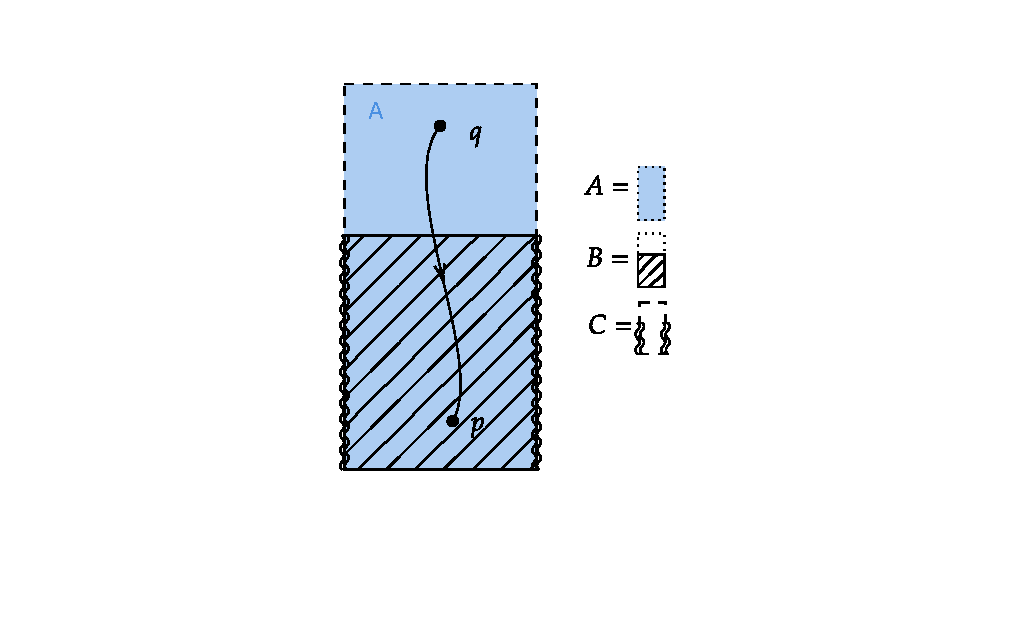
\includegraphics{Text/Pictures/general Proof idea.pdf}
	
	From the perspective of K-theory a regular index pair for a critical point is the same as a sphere with the dimension beeing the index of said critical point. To see this just use a small index pair in a Morse chart (they are all homotopic anyway), collaps the stable part and quotiend by the exit set. By doing this we get the communative diagramm:
	\begin{center}
		% https://tikzcd.yichuanshen.de/#N4Igdg9gJgpgziAXAbVABwnAlgFyxMJZABgBpiBdUkANwEMAbAVxiRAGkA9YAawFoAjAF8AFACFSAYQCUIIaXSZc+QigHkqtRizZdeogIKkxs+Yux4CRMgM31mrRB279hIgMovBQ0wpAYLFSJ1W2p7HSc9HlFPXm9fc2UrFDIAJjttR2d9DxcfOU0YKABzeCJQADMAJwgAWyQyEBwIJFSzEGq6pHUmlsQAZnbO+sRG5u6wzLYAHWnYBhw6AH1gHCqsNAYYITk-YdbqcYGhmpGAFkO+wb3Tg96kM6EKISA
		\begin{tikzcd}
			{K^{k-1}(B,C)} \arrow[d] \arrow[r, "\delta_{triple}"] & {K^{k}(A,B)} \arrow[d] \\
			K^{k-1}(S^{k-1}) \arrow[r] \arrow[d]                  & K^{k}(S^{k-1})         \\
			K^{k}(S^{k}) \arrow[ru]                               &                       
		\end{tikzcd}
	\end{center} And as a map between K Groups of spheres, we know that this map corresponds to the question of orientation. Now we have the maps 
	\begin{enumerate}[(a)]
		\item $S^k\to S\vee (B\big/ C)$ induced from an orientation in the unstable manifold arround $p$ together with $-\grad(f)(x_i)$ where $x_i\in W(q\to p)$. 
		\item $S^k \to (A\big/ B)$ induced from an orientation in the unstable manifold arround $q$. 
	\end{enumerate}
	And hence the diagram 
	\begin{center}
		% https://tikzcd.yichuanshen.de/#N4Igdg9gJgpgziAXAbVABwnAlgFyxMJZABgBpiBdUkANwEMAbAVxiRAGkA9YAawF8AFAGUAOiJowYAAgEAhUgGEAlEpB9S6TLnyEUARlJ6qtRizZdegoZx6r1m7HgJEATOWP1mrRB278BAIKksnbGMFAA5vBEoABmAE4QALZIZCA4EEhuJl5sYrAMOHQA+sA48VhoDDB8ahogCclIBumZiC72DYkpiC0ZqXwUfEA
		\begin{tikzcd}
			{K^{k}(S\vee (B,C))} \arrow[rr, "\delta_{triple}"] &                                  & {K^{k}(A,B)} \\
			& K^{k}(S^k) \arrow[ru] \arrow[lu] &             
		\end{tikzcd}
	\end{center}
	The map now factors over The K-Group of a bouquette of $k$-spheres generated over the connecting flow lines. In each such sphere the comparison of orientations happens.
\end{Iprove}

Bevore we start proving this we need the lemma: 

\begin{lemma}\label{lem: The Main Lemma Np is tubular}
	We work in a compact, riemanian, orientable, smooth Manifold $(M,g)$ of dimension $m$ together with a Morse-Smale funktion 
	\begin{align}
		f: M\to \R
	\end{align}
	We assume that $q$ is a critical point of index $k+1$ and $p$ is a critical point of index $k$. we define $f(q)=b$ and $f(p)=a$ and assume that there is no critical point in $f^{-1}(a,b)\subseteq M$. We define the sub and superlevelsets 
	\begin{align}
		M^t:=\{ x\in M | f(x)\leq t \} \quad \text{and}\quad M_t:=\{ x\in M | f(x)\geq t \} \, ,
	\end{align} and the constants 
	\begin{align}
		c \in (a,b) \quad , \quad \epsilon >0 \text{ small } \quad,\quad T>0 \text{ big .}
	\end{align} With this we define the sets: 
	\begin{align}
		N_q  & \coloneq    \{ x\in M_c |f(\phi_{-T}(x))  \leq b+ \epsilon  \}   \, ,  \\
		L_q  & \coloneq    \{ x\in N_q |f(x)             =    c            \}    \, , \\
		N_p  & \coloneq    \{ x\in M^c |f(\phi_T(x))     \geq a-\epsilon   \}    \, , \\
		L_p  & \coloneq    \{ x\in N_p |f( \phi_T(x))    =    a-\epsilon   \} \, ,
	\end{align} and finally: 
	\begin{align}
		C  & \coloneq  N_p \cup N_q  \, ,                     \\
		B  & \coloneq  N_p \cup L_q   \, ,                   \\
		A  & \coloneq  L_p \cup \mathring{(L_q-N_p)} \, .
	\end{align}
	
	We claim that 
	\begin{enumerate}
		\item $(N_q,L_q)$ is a regular index pair for $q$\, . \label{lem: enum: 1}
		\item $(C,B)$ is an index pair for $q$\, .\label{lem: enum: 2}
		\item $(N_p,L_p)$ is a regular index pair for $p$\, .\label{lem: enum: 3}
		\item $(B,A)$ is an index pair for $p$\, .\label{lem: enum: 4}
		\item $N_p$ is a tubular neighbourhood of $W(\to p)\cap M^c$.\label{lem: enum: 5}
	\end{enumerate}
\end{lemma}

\begin{Iprove}
	The statements \ref{lem: enum: 1}-\ref{lem: enum: 4} are easy to proof by the definitions. The regularity can be derived from a general fact for pairs $(X,Y)$ in metric spaces: If $Y$ is closed in $X$ and there is a neighbourhood of $Y$ that is open in $X$ such that $Y$ is a strong deformation retract of $U$. So the only thing left to show is, that $N_p$ is a tubular neighbourhood. In \cite{Salamon1990} in the proof of lemma 3.2 Salamon claims this to be true without a proof (page 119 in the attached source). Similar, in \cite{banyaga2004lectures} Banyaga claims this (also without any argument).
	The Set $N_p$ is sketched in the figure below. 
	The Idea of the proove is as follows: By increasing $T$ (or decreasing $\epsilon$) we can assume $N_p$ to be an arbitrary small neighbourhood of $W(q\to) \cap M^c$. Now using the flow we can push $N_p$ close to $p$ ($\phi_N(N_p)$ for big $N$ ), where we use a tubular nieghbourhood embedding $J$ that overlapps $N_p$. We now need to proof that we can reduce the radii of the fibers in the domain of $J$ in a smooth way such that $J$ actually becomes a embedding onto the $N_p$ (that we pushed close to $p$). For this we will make use of the lambda lemma (in an improved version), which lets us induce a metric from the unstable tangend space of $P$ into the fiberes of $J$ (since they are transversal to the stable set). With this metric we can finally smoothly reduce the radii of our domain of $J$ to end up with the statement, that $\phi_N(N_p)$ is a tubular neighbourhood of a small part of the stable set of $p$ and hence $N_p$ also. The prove is given as an appendix in section \ref{section: Np tubular neighbourhood proove}.
\end{Iprove}
\begin{center}
	
	
	\tikzset{every picture/.style={line width=0.75pt}} %set default line width to 0.75pt        
	\resizebox{\linewidth}{!}{%
		
		
		
		\tikzset{every picture/.style={line width=0.75pt}} %set default line width to 0.75pt      
		
		\tikzset{every picture/.style={line width=0.75pt}} %set default line width to 0.75pt        
		
		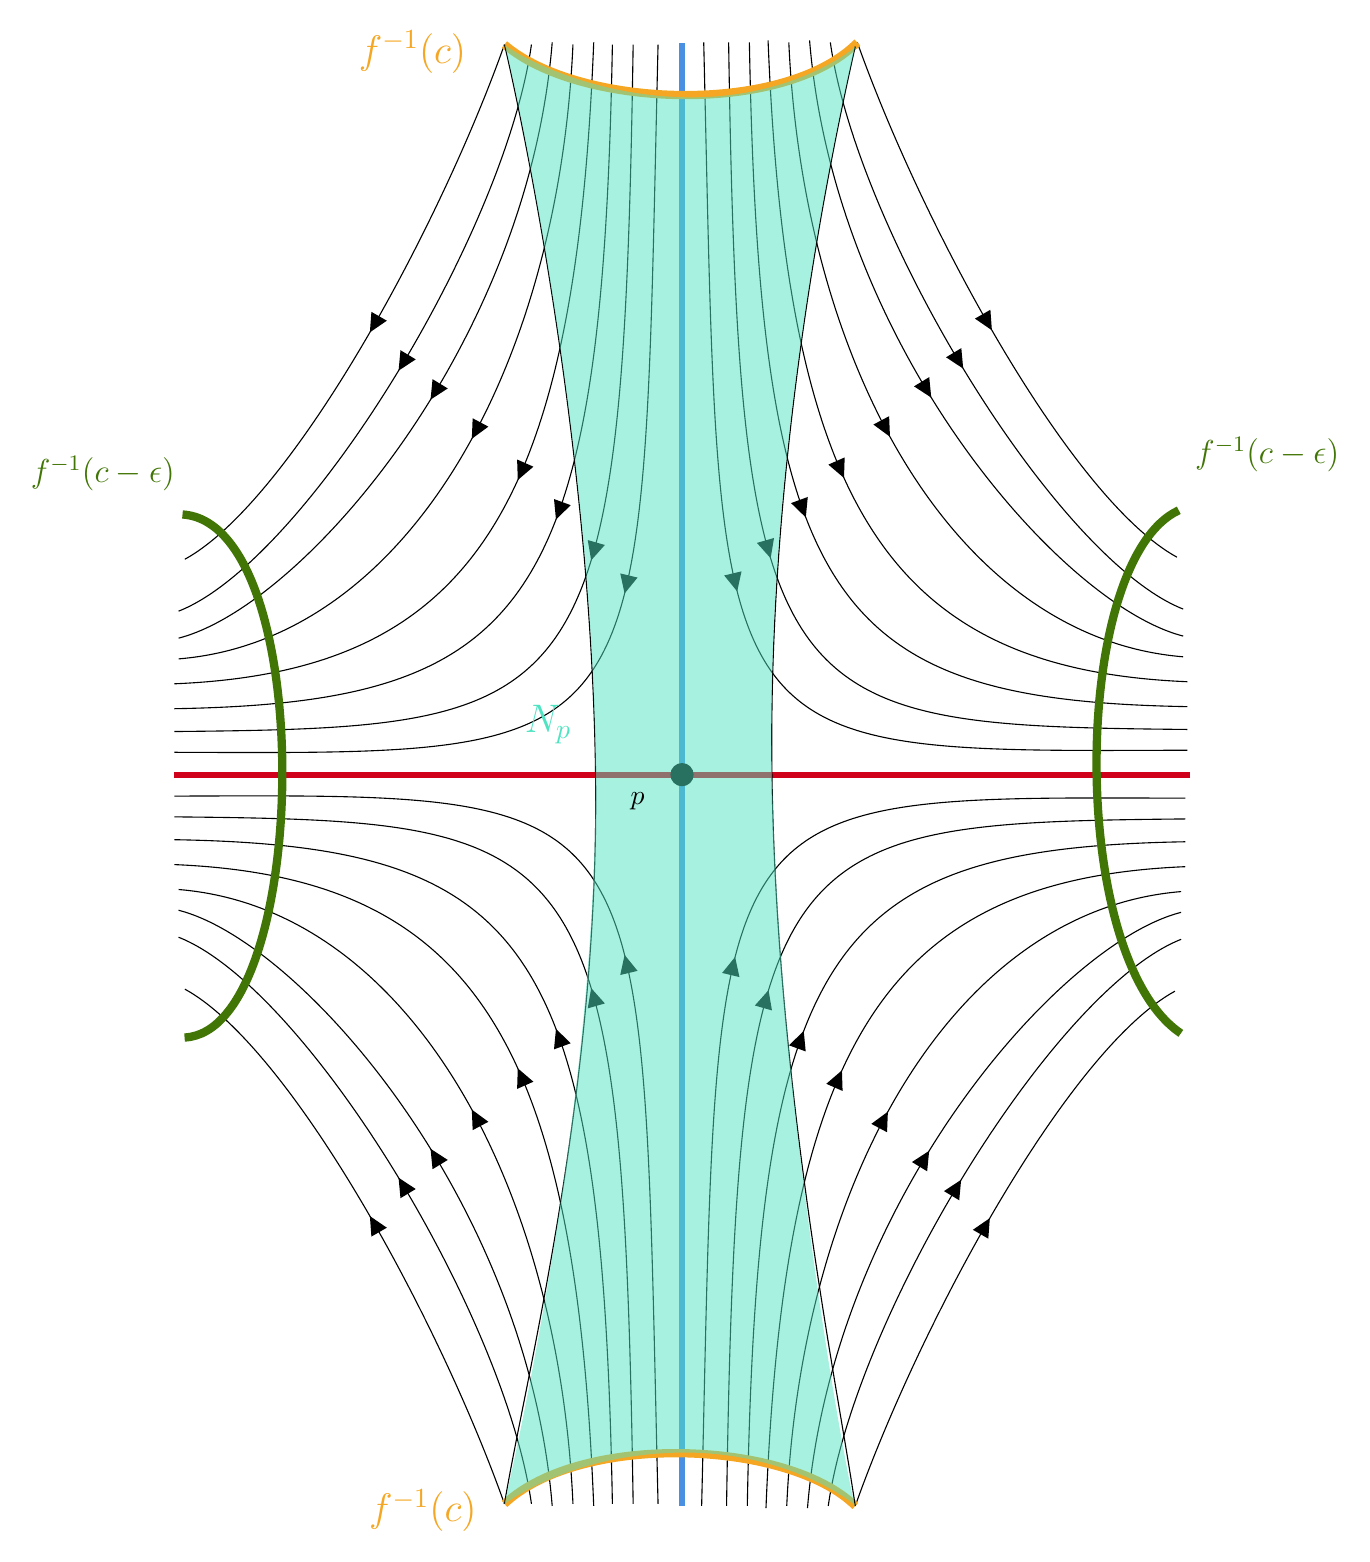
\begin{tikzpicture}[x=0.75pt,y=0.75pt,yscale=-1,xscale=1]
			%uncomment if require: \path (0,843); %set diagram left start at 0, and has height of 843
			
			%Straight Lines [id:da11875089429305197] 
			\draw [color={rgb, 255:red, 74; green, 144; blue, 226 }  ,draw opacity=1 ][line width=2.25]    (329,31.6) -- (329,736.43) ;
			%Straight Lines [id:da5325201497809933] 
			\draw [color={rgb, 255:red, 208; green, 2; blue, 27 }  ,draw opacity=1 ][line width=2.25]    (84.42,384.02) -- (573.58,384.02) ;
			%Shape: Circle [id:dp07579894054308489] 
			\draw  [draw opacity=0][fill={rgb, 255:red, 0; green, 0; blue, 0 }  ,fill opacity=1 ] (323.4,384.02) .. controls (323.4,380.92) and (325.91,378.42) .. (329,378.42) .. controls (332.09,378.42) and (334.6,380.92) .. (334.6,384.02) .. controls (334.6,387.11) and (332.09,389.62) .. (329,389.62) .. controls (325.91,389.62) and (323.4,387.11) .. (323.4,384.02) -- cycle ;
			%Curve Lines [id:da1665503577346341] 
			\draw    (339.45,31.25) .. controls (347.8,378.2) and (336.45,373.05) .. (572.45,372.25) ;
			\draw [shift={(355.57,295.75)}, rotate = 256.55] [fill={rgb, 255:red, 0; green, 0; blue, 0 }  ][line width=0.08]  [draw opacity=0] (8.93,-4.29) -- (0,0) -- (8.93,4.29) -- cycle    ;
			%Curve Lines [id:da7994448259938868] 
			\draw    (351.45,31.25) .. controls (356.45,355.25) and (373.45,360.25) .. (572.45,362.25) ;
			\draw [shift={(371.68,279.76)}, rotate = 253.92] [fill={rgb, 255:red, 0; green, 0; blue, 0 }  ][line width=0.08]  [draw opacity=0] (8.93,-4.29) -- (0,0) -- (8.93,4.29) -- cycle    ;
			%Curve Lines [id:da558792425961241] 
			\draw    (361.45,31.25) .. controls (366.45,302.25) and (401.45,348.25) .. (572.45,351.25) ;
			\draw [shift={(388.63,260.1)}, rotate = 249.87] [fill={rgb, 255:red, 0; green, 0; blue, 0 }  ][line width=0.08]  [draw opacity=0] (8.93,-4.29) -- (0,0) -- (8.93,4.29) -- cycle    ;
			%Curve Lines [id:da5211576581151481] 
			\draw    (370.45,30.25) .. controls (379.45,254.25) and (428.45,333.25) .. (572.45,339.25) ;
			\draw [shift={(407.03,241.09)}, rotate = 246.23] [fill={rgb, 255:red, 0; green, 0; blue, 0 }  ][line width=0.08]  [draw opacity=0] (8.93,-4.29) -- (0,0) -- (8.93,4.29) -- cycle    ;
			%Curve Lines [id:da39021575553782684] 
			\draw    (380.45,31.25) .. controls (387.45,187.25) and (460.45,318.25) .. (570.45,327.25) ;
			\draw [shift={(429.18,221.22)}, rotate = 242] [fill={rgb, 255:red, 0; green, 0; blue, 0 }  ][line width=0.08]  [draw opacity=0] (8.93,-4.29) -- (0,0) -- (8.93,4.29) -- cycle    ;
			%Curve Lines [id:da6126506516051217] 
			\draw    (390.45,30.25) .. controls (402.45,177.25) and (511.45,302.25) .. (570.45,317.25) ;
			\draw [shift={(449.07,202.35)}, rotate = 238.74] [fill={rgb, 255:red, 0; green, 0; blue, 0 }  ][line width=0.08]  [draw opacity=0] (8.93,-4.29) -- (0,0) -- (8.93,4.29) -- cycle    ;
			%Curve Lines [id:da24082042581971141] 
			\draw    (400.45,31.25) .. controls (413.45,123.25) and (509.45,280.25) .. (570.45,304.25) ;
			\draw [shift={(464.47,188.39)}, rotate = 239.04] [fill={rgb, 255:red, 0; green, 0; blue, 0 }  ][line width=0.08]  [draw opacity=0] (8.93,-4.29) -- (0,0) -- (8.93,4.29) -- cycle    ;
			%Curve Lines [id:da5298362087143788] 
			\draw    (413.45,31.25) .. controls (445.45,121.25) and (516.45,251.25) .. (567.45,279.25) ;
			\draw [shift={(478.29,169.92)}, rotate = 240.15] [fill={rgb, 255:red, 0; green, 0; blue, 0 }  ][line width=0.08]  [draw opacity=0] (8.93,-4.29) -- (0,0) -- (8.93,4.29) -- cycle    ;
			
			%Curve Lines [id:da21918221686589523] 
			\draw    (317.45,32.25) .. controls (309.1,379.2) and (320.45,374.05) .. (84.45,373.25) ;
			\draw [shift={(301.33,296.75)}, rotate = 283.45] [fill={rgb, 255:red, 0; green, 0; blue, 0 }  ][line width=0.08]  [draw opacity=0] (8.93,-4.29) -- (0,0) -- (8.93,4.29) -- cycle    ;
			%Curve Lines [id:da34745008178206616] 
			\draw    (305.45,32.25) .. controls (300.45,356.25) and (283.45,361.25) .. (84.45,363.25) ;
			\draw [shift={(285.22,280.76)}, rotate = 286.08] [fill={rgb, 255:red, 0; green, 0; blue, 0 }  ][line width=0.08]  [draw opacity=0] (8.93,-4.29) -- (0,0) -- (8.93,4.29) -- cycle    ;
			%Curve Lines [id:da8640093846313118] 
			\draw    (295.45,32.25) .. controls (290.45,303.25) and (255.45,349.25) .. (84.45,352.25) ;
			\draw [shift={(268.27,261.1)}, rotate = 290.13] [fill={rgb, 255:red, 0; green, 0; blue, 0 }  ][line width=0.08]  [draw opacity=0] (8.93,-4.29) -- (0,0) -- (8.93,4.29) -- cycle    ;
			%Curve Lines [id:da925990106139973] 
			\draw    (286.45,31.25) .. controls (277.45,255.25) and (228.45,334.25) .. (84.45,340.25) ;
			\draw [shift={(249.87,242.09)}, rotate = 293.77] [fill={rgb, 255:red, 0; green, 0; blue, 0 }  ][line width=0.08]  [draw opacity=0] (8.93,-4.29) -- (0,0) -- (8.93,4.29) -- cycle    ;
			%Curve Lines [id:da08743123557319321] 
			\draw    (276.45,32.25) .. controls (269.45,188.25) and (196.45,319.25) .. (86.45,328.25) ;
			\draw [shift={(227.72,222.22)}, rotate = 298] [fill={rgb, 255:red, 0; green, 0; blue, 0 }  ][line width=0.08]  [draw opacity=0] (8.93,-4.29) -- (0,0) -- (8.93,4.29) -- cycle    ;
			%Curve Lines [id:da08430775562121551] 
			\draw    (266.45,31.25) .. controls (254.45,178.25) and (145.45,303.25) .. (86.45,318.25) ;
			\draw [shift={(207.83,203.35)}, rotate = 301.26] [fill={rgb, 255:red, 0; green, 0; blue, 0 }  ][line width=0.08]  [draw opacity=0] (8.93,-4.29) -- (0,0) -- (8.93,4.29) -- cycle    ;
			%Curve Lines [id:da38820398572752524] 
			\draw    (256.45,32.25) .. controls (243.45,124.25) and (147.45,281.25) .. (86.45,305.25) ;
			\draw [shift={(192.43,189.39)}, rotate = 300.96] [fill={rgb, 255:red, 0; green, 0; blue, 0 }  ][line width=0.08]  [draw opacity=0] (8.93,-4.29) -- (0,0) -- (8.93,4.29) -- cycle    ;
			%Curve Lines [id:da5677669307058717] 
			\draw    (243.45,32.25) .. controls (211.45,122.25) and (140.45,252.25) .. (89.45,280.25) ;
			\draw [shift={(178.61,170.92)}, rotate = 299.85] [fill={rgb, 255:red, 0; green, 0; blue, 0 }  ][line width=0.08]  [draw opacity=0] (8.93,-4.29) -- (0,0) -- (8.93,4.29) -- cycle    ;
			
			%Curve Lines [id:da5375642083324416] 
			\draw    (338.45,736.36) .. controls (346.8,389.41) and (335.45,394.56) .. (571.45,395.36) ;
			\draw [shift={(354.57,471.87)}, rotate = 103.45] [fill={rgb, 255:red, 0; green, 0; blue, 0 }  ][line width=0.08]  [draw opacity=0] (8.93,-4.29) -- (0,0) -- (8.93,4.29) -- cycle    ;
			%Curve Lines [id:da5126738644229648] 
			\draw    (350.45,736.36) .. controls (355.45,412.36) and (372.45,407.36) .. (571.45,405.36) ;
			\draw [shift={(370.68,487.86)}, rotate = 106.08] [fill={rgb, 255:red, 0; green, 0; blue, 0 }  ][line width=0.08]  [draw opacity=0] (8.93,-4.29) -- (0,0) -- (8.93,4.29) -- cycle    ;
			%Curve Lines [id:da5839119584885231] 
			\draw    (360.45,736.36) .. controls (365.45,465.36) and (400.45,419.36) .. (571.45,416.36) ;
			\draw [shift={(387.63,507.52)}, rotate = 110.13] [fill={rgb, 255:red, 0; green, 0; blue, 0 }  ][line width=0.08]  [draw opacity=0] (8.93,-4.29) -- (0,0) -- (8.93,4.29) -- cycle    ;
			%Curve Lines [id:da975815253328843] 
			\draw    (369.45,737.36) .. controls (378.45,513.36) and (427.45,434.36) .. (571.45,428.36) ;
			\draw [shift={(406.03,526.52)}, rotate = 113.77] [fill={rgb, 255:red, 0; green, 0; blue, 0 }  ][line width=0.08]  [draw opacity=0] (8.93,-4.29) -- (0,0) -- (8.93,4.29) -- cycle    ;
			%Curve Lines [id:da9314613290760876] 
			\draw    (379.45,736.36) .. controls (386.45,580.36) and (459.45,449.36) .. (569.45,440.36) ;
			\draw [shift={(428.18,546.4)}, rotate = 118] [fill={rgb, 255:red, 0; green, 0; blue, 0 }  ][line width=0.08]  [draw opacity=0] (8.93,-4.29) -- (0,0) -- (8.93,4.29) -- cycle    ;
			%Curve Lines [id:da09174306781681929] 
			\draw    (389.45,737.36) .. controls (401.45,590.36) and (510.45,465.36) .. (569.45,450.36) ;
			\draw [shift={(448.07,565.26)}, rotate = 121.26] [fill={rgb, 255:red, 0; green, 0; blue, 0 }  ][line width=0.08]  [draw opacity=0] (8.93,-4.29) -- (0,0) -- (8.93,4.29) -- cycle    ;
			%Curve Lines [id:da21494064860512774] 
			\draw    (399.45,736.36) .. controls (412.45,644.36) and (508.45,487.36) .. (569.45,463.36) ;
			\draw [shift={(463.47,579.22)}, rotate = 120.96] [fill={rgb, 255:red, 0; green, 0; blue, 0 }  ][line width=0.08]  [draw opacity=0] (8.93,-4.29) -- (0,0) -- (8.93,4.29) -- cycle    ;
			%Curve Lines [id:da506519829239\end{proo7652] 
				\draw    (412.45,736.36) .. controls (444.45,646.36) and (515.45,516.36) .. (566.45,488.36) ;
				\draw [shift={(477.29,597.7)}, rotate = 119.85] [fill={rgb, 255:red, 0; green, 0; blue, 0 }  ][line width=0.08]  [draw opacity=0] (8.93,-4.29) -- (0,0) -- (8.93,4.29) -- cycle    ;
				
				%Curve Lines [id:da3880154567702636] 
				\draw    (317.45,735.36) .. controls (309.1,388.41) and (320.45,393.56) .. (84.45,394.36) ;
				\draw [shift={(301.33,470.87)}, rotate = 76.55] [fill={rgb, 255:red, 0; green, 0; blue, 0 }  ][line width=0.08]  [draw opacity=0] (8.93,-4.29) -- (0,0) -- (8.93,4.29) -- cycle    ;
				%Curve Lines [id:da9327211409936709] 
				\draw    (305.45,735.36) .. controls (300.45,411.36) and (283.45,406.36) .. (84.45,404.36) ;
				\draw [shift={(285.22,486.86)}, rotate = 73.92] [fill={rgb, 255:red, 0; green, 0; blue, 0 }  ][line width=0.08]  [draw opacity=0] (8.93,-4.29) -- (0,0) -- (8.93,4.29) -- cycle    ;
				%Curve Lines [id:da09647590503157577] 
				\draw    (295.45,735.36) .. controls (290.45,464.36) and (255.45,418.36) .. (84.45,415.36) ;
				\draw [shift={(268.27,506.52)}, rotate = 69.87] [fill={rgb, 255:red, 0; green, 0; blue, 0 }  ][line width=0.08]  [draw opacity=0] (8.93,-4.29) -- (0,0) -- (8.93,4.29) -- cycle    ;
				%Curve Lines [id:da15668737739736305] 
				\draw    (286.45,736.36) .. controls (277.45,512.36) and (228.45,433.36) .. (84.45,427.36) ;
				\draw [shift={(249.87,525.52)}, rotate = 66.23] [fill={rgb, 255:red, 0; green, 0; blue, 0 }  ][line width=0.08]  [draw opacity=0] (8.93,-4.29) -- (0,0) -- (8.93,4.29) -- cycle    ;
				%Curve Lines [id:da5883237308999977] 
				\draw    (276.45,735.36) .. controls (269.45,579.36) and (196.45,448.36) .. (86.45,439.36) ;
				\draw [shift={(227.72,545.4)}, rotate = 62] [fill={rgb, 255:red, 0; green, 0; blue, 0 }  ][line width=0.08]  [draw opacity=0] (8.93,-4.29) -- (0,0) -- (8.93,4.29) -- cycle    ;
				%Curve Lines [id:da9204033290837756] 
				\draw    (266.45,736.36) .. controls (254.45,589.36) and (145.45,464.36) .. (86.45,449.36) ;
				\draw [shift={(207.83,564.26)}, rotate = 58.74] [fill={rgb, 255:red, 0; green, 0; blue, 0 }  ][line width=0.08]  [draw opacity=0] (8.93,-4.29) -- (0,0) -- (8.93,4.29) -- cycle    ;
				%Curve Lines [id:da49739155745577546] 
				\draw    (256.45,735.36) .. controls (243.45,643.36) and (147.45,486.36) .. (86.45,462.36) ;
				\draw [shift={(192.43,578.22)}, rotate = 59.04] [fill={rgb, 255:red, 0; green, 0; blue, 0 }  ][line width=0.08]  [draw opacity=0] (8.93,-4.29) -- (0,0) -- (8.93,4.29) -- cycle    ;
				%Curve Lines [id:da32213499249738287] 
				\draw    (243.45,735.36) .. controls (211.45,645.36) and (140.45,515.36) .. (89.45,487.36) ;
				\draw [shift={(178.61,596.7)}, rotate = 60.15] [fill={rgb, 255:red, 0; green, 0; blue, 0 }  ][line width=0.08]  [draw opacity=0] (8.93,-4.29) -- (0,0) -- (8.93,4.29) -- cycle    ;
				
				
				%Curve Lines [id:da05541171078629925] 
				\draw [color={rgb, 255:red, 245; green, 166; blue, 35 }  ,draw opacity=1 ][line width=3]    (243.45,32.25) .. controls (279.42,63.08) and (378.33,66.67) .. (413.45,31.25) ;
				%Curve Lines [id:da4989004892868002] 
				\draw [color={rgb, 255:red, 245; green, 166; blue, 35 }  ,draw opacity=1 ][line width=3]    (243.45,735.36) .. controls (280.33,700.67) and (380.33,704.67) .. (412.45,736.36) ;
				%Curve Lines [id:da44411839842500755] 
				\draw [color={rgb, 255:red, 65; green, 117; blue, 5 }  ,draw opacity=1 ][line width=3]    (88.33,258.67) .. controls (154.22,262.97) and (150.33,507.67) .. (89.33,510.67) ;
				%Curve Lines [id:da05367202270104565] 
				\draw [color={rgb, 255:red, 65; green, 117; blue, 5 }  ,draw opacity=1 ][line width=3]    (568.33,256.67) .. controls (516.33,280.67) and (514.33,471.67) .. (569.33,508.67) ;
				%Curve Lines [id:da7969530986481941] 
				\draw    (243.45,32.25) .. controls (254.33,78.67) and (285.1,230.49) .. (287.33,382.67) .. controls (289.57,534.85) and (253.34,675.31) .. (243.45,735.36) ;
				%Curve Lines [id:da5283140439270424] 
				\draw    (412.45,33.25) .. controls (400.33,86.67) and (370.1,232.49) .. (372.33,384.67) .. controls (374.57,536.85) and (404.33,680.67) .. (412.45,736.36) ;
				
				%Shape: Polygon Curved [id:ds3817941045439226] 
				\draw  [draw opacity=0][fill={rgb, 255:red, 80; green, 227; blue, 194 }  ,fill opacity=0.5 ] (243.45,735.36) .. controls (243.39,735.01) and (288.33,547.67) .. (287.33,382.67) .. controls (286.33,217.67) and (244.39,31.96) .. (243.45,32.25) .. controls (242.51,32.54) and (278.33,56.67) .. (330.33,57.67) .. controls (382.33,58.67) and (412.39,33.99) .. (412.45,33.25) .. controls (412.51,32.51) and (368.33,212.67) .. (372.33,384.67) .. controls (376.33,556.67) and (411.01,736.21) .. (412.45,736.36) .. controls (413.89,736.52) and (381.33,709.67) .. (327.33,710.67) .. controls (273.33,711.67) and (243.51,735.72) .. (243.45,735.36) -- cycle ;
				
				% Text Node
				\draw (303,391.4) node [anchor=north west][inner sep=0.75pt]    {$p$};
				% Text Node
				\draw (172,24.4) node [anchor=north west][inner sep=0.75pt]  [font=\Large,color={rgb, 255:red, 245; green, 166; blue, 35 }  ,opacity=1 ]  {$f^{-1}( c)$};
				% Text Node
				\draw (177,727.07) node [anchor=north west][inner sep=0.75pt]  [font=\Large,color={rgb, 255:red, 245; green, 166; blue, 35 }  ,opacity=1 ]  {$f^{-1}( c)$};
				% Text Node
				\draw (14,229.4) node [anchor=north west][inner sep=0.75pt]  [font=\large,color={rgb, 255:red, 65; green, 117; blue, 5 }  ,opacity=1 ]  {$f^{-1}( c-\epsilon )$};
				% Text Node
				\draw (575,220.4) node [anchor=north west][inner sep=0.75pt]  [font=\large,color={rgb, 255:red, 65; green, 117; blue, 5 }  ,opacity=1 ]  {$f^{-1}( c-\epsilon )$};
				% Text Node
				\draw (252,349.4) node [anchor=north west][inner sep=0.75pt]  [font=\Large,color={rgb, 255:red, 80; green, 227; blue, 194 }  ,opacity=1 ]  {$N_{p}$};
				
				
			\end{tikzpicture}
			
			
		}
	\end{center}
	
	The same arguments work to show that $N_q$ is a tubular neighbourhood of $W(q\to)\cap M_c$, by replacing $f$ with $-f$. Furthermore, we can assume, that the $V_j$ from below are fibers in the normal neighbourhood. This can be realized, since $V_j$ intersect transversal and by trivialization we have a global fram of the bundel and hence can smoothly rescale the embedding along the frame to get that $V_j$ is the image of the fibre above $x_j$. 
	
	
	
	
	
	
	
	
	
	
	
	\begin{proof}[Proof of Theorem \ref{thm: commuting connecting homomorphism}]
		We first notice, that we have the map of triples given by the inclusion:
		\begin{align*}
			\left( ~W(q\to)\cap N_q ~,~S(q\to)~,~S(q\to ) \setminus \bigcup\limits_jV_j ~\right) \to (C,B,A)
		\end{align*} and hence by naturalitiy we have the diagram, where the top square commutes:
		\begin{fdiagram}
			% https://tikzcd.yichuanshen.de/#N4Igdg9gJgpgziAXAbVABwnAlgFyxMJZABgBpiBdUkANwEMAbAVxiRAGkA9YAWgB0+DOgFsARlDoB9NAF8BDGADMcyAAQAhUgEFVAgE5YA5gAscFEDNLpMufIRQBGclVqMWbLr3kjxUgI5ygkoqAMKkGrp8BiZmFlYgGNh4BERkDi70zKyIHNz8gj4S0oEKymoAygAUfgI4EACUpFU1fHX1AnAwOMJYYExwkaJGAMZMaPJYPThwkgBWkb14lQBqc-WR0abmltZJdkRO6dSZ7jme+UJiRQHywcgA6tW1DQLDdGiqAHLSTU+tDRsjFs4rtbCkUGQAEwZNzZXJeApXKSyW5lVSrWakARoOh6PCMdFzQExbYuGBQQzwIigRR6CDCJBkEB1JBOEBCUQwBgABRsyXs7OCIGOsLYAlgDBwUmAOAMaAUMk4DhBIFp9MZ1BZiEhIqybCwkmAmi0ioAVCq1QzEGytQBmXWnEAG4BhdRmi10q065kQJD21x6nLirlSw2yrDymCKyEe9XazW+xAAFgdcINs045uoHK5vL24JAmxwwpAcGMWGUSEhO1VnqQKZ9ftTYr4EqlnFmYblCpLOZ5fP2OSLsatDa13pOcOGc0zvbonP7+YFw5kFBkQA
			\begin{tikzcd}
				{K^{-\lambda_p}\left[ B,A \right]} \arrow[r, "\delta_{triple}^1"] \arrow[d, "{i_{B,A}^*}"]                                                            & {K^{-\lambda_q}\left[C, B \right]} \arrow[d, "{i_{C,B}^*}"] \\
				{K^{-\lambda_p}\left[ S(q\to),S(q\to)\setminus \bigcup\limits_j \inti(V_j) \right]} \arrow[r, "\delta_{triple}^2"] \arrow[d, "i_j^*"', shift right=2] & {K^{-\lambda_q}\left[W(q\to)\cap N_p,S(q\to) \right]}       \\
				{K^{-\lambda_p}\left[ V_j,\partial V_j \right]} \arrow[ru, "\delta^j_{triple}"'] \arrow[u, "c_j^*"']                                                  &                                                            
			\end{tikzcd} 
		\end{fdiagram}
		\noindent	Furthermore, in this diagram the tuple $\left(K^{-\lambda_p}\left[ S(q\to),S(q\to)\setminus \bigcup\limits_j \inti(V_j) \right],\left(c_j^*\right)_j\right)$ is a coproduct, and we define  $\delta^j_{triple}\coloneq \delta^2_{triple}\circ c_j^*$. Then we have that 
		\begin{equation*}
			\delta^2_ {triple}=\sum_j\delta^j_{triple}\circ i_j^*
		\end{equation*}
		Since $i_{C,B}^*$ is an isomorphism (since $W(q\to \cap N_p$ is a deformation retract of $C$ and the collaps collapses $B$ to $S(q\to)$), we have that 
		\begin{equation} \label{eq: Delta in terms of delta j}
			\Delta(\alpha_q)=\delta^1_{triple}(\alpha_q)=i^*_{C,B}\circ \sum_j\delta^j_{triple}\circ i_j^* \circ i^*_{B,A}(\alpha_q)
		\end{equation}
		
		The map $\delta^2_{triple}$ is defined as the composition:
		\begin{fdiagram} \label{diag: Definitino of delta j}
			\begin{adjustbox}{max width=\textwidth}
				% https://tikzcd.yichuanshen.de/#N4Igdg9gJgpgziAXAbVABwnAlgFyxMJZABgBoBGAXVJADcBDAGwFcYkQBpAPWAFoAdfo3oBbAEZR6AfTQBfQYxgAzHMgAEAZQAUAR0E4IASlLa9-A4cFwYOEVjDM4awWKwBzAMbM0CrHZxwUgBWzvz2eFoAasGGoQBO7gAWOJQgsqTomLj4hChkAEzUdEys7Nx8CqIS0nIKyqqauvpG8UkpaRkgGNh4BETkpIU0DCxsiJw8AkJVkjIA1OTyQvXIGlLkgrQwMI1mFq1uyanpmT05RPmDRSOl4+VTwuKzaAtLiirIAOpN5kaCHvQ0GoAHIyf7eNQAYXWdRUWl2zUs-AShxwxm+ez+-ABQNBQMEKKOHVO2T6KAAzFdhiUxhMKtMnjVXrDVBjEf9ASCwdiIdCNss4QjfkjCWiCW1jp1uqTcshKVRqaMypNKoypDo3is2cKObiZCYfvtxajJSTerKyMRrjTlfTHtUZJqPmpokFSII0PQ4ngmC7ggcibIijAoG54ERQEo4hAREgyCADEgBsUleMsOsuAAqYkgKMxpM0ROIS4p24gRJZ9Y5vOx4uFiBISml2mJKT5LPV6O1ptFgAsirL6fb2ZOua7SH7CYbiAArAPaS4bPR-lg4h5QjgYAAPHDAHAJWiyKTAPmmRGyTv5xDxotz5vsQSwRg4ehcfLH-dYNCKC+jmtIAA2es43ndgPGCDsg1kIA
				\begin{tikzcd}
					{K^{-\lambda_p}\left[ V_j,\partial V_j \right]} \arrow[d, "c_j^*"]                                                                      &                                                                    &                                                                                                                 &                                                                                                                              \\
					{K^{-\lambda_p}\left[ S(q\to),S(q\to)\setminus \bigcup\limits_j \inti(V_j) \right]} \arrow[d, "i_1^*"] \arrow[rrr, "\delta^2_{triple}"] &                                                                    &                                                                                                                 & {K^{-\lambda_q}\left[W(q\to)\cap N_p,S(q\to) \right]}                                                                        \\
					{K^{-\lambda_p}\left[ S(q\to) \right]} \arrow[r, "h^*_1"]                                                                               & {K^{-\lambda_p+1}\left[S_1\vee S(q\to) \right]} \arrow[r, "h_2^*"] & {K^{-\lambda_p+1}\left[W(q\to)\cap N_p\cup C_1\left( S(q\to)\right),W(q\to)\cap N_p \right]} \arrow[r, "i_2^*"] & {K^{-\lambda_p+1}\left[W(q\to)\cap N_p\cup C_1\left( S(q\to)\right)\right]} \arrow[u, "\beta\circ \text{triv}_{C_1S(q\to)}"]
				\end{tikzcd}
			\end{adjustbox}
		\end{fdiagram}
		
		The downwards maps in the theorem are the induction of the canonical generators. This is done by the following assignement
		
		
		
		Now the composition \begin{equation*}
			h_1*i_1*\circ c_j*: K^{-\lambda_p}\left[ V_j,\partial V_j \right] \to K^{-\lambda_p+1}\left[S_1\vee S(q\to) \right]
		\end{equation*} can be simplified by the map
		\begin{equation*}
			l^*:	K^{-\lambda_p}\left[ V_j,\partial V_j \right]=K^{-\lambda_p+1}\left[S_1\vee\left( V_j,\partial V_j\right) \right] \to K^{-\lambda_p+1}\left[S_1\vee S(q\to) \right]
		\end{equation*} where l is the collapsing map.
		\begin{align*}
			l:S_1\vee S(q\to)  \to S_1\vee\left( V_j,\partial V_j\right)\\
			(t,x)\mapsto (t,\overline{x})
		\end{align*} So now we are in the following situation: 
		\begin{fdiagram}
			\begin{adjustbox}{max width=\textwidth}
				% % https://tikzcd.yichuanshen.de/#N4Igdg9gJgpgziAXAbVABwnAlgFyxMJZABgBpiBdUkANwEMAbAVxiRAGkA9YAWgB0+DOgFsARlDoB9NAF8BDGADMcyAGqSAVqQFo6AJzyMABOo1GBerAHMAFjgogZpdJlz5CKAEzkqtRizYuXnkRcSkARzlBJRUAdQAKcPM+HAgjAEoBAGM6NCMAOWlSAGVEgVTMvktbe0dnEAxsPAIib09femZWRA5ufkFQiWkeAEYohWVkAWE6HBtRUWBimW4QsSG0AGox5Oq7BycXJvciMnbqToCeoP6hdak0UfGYqb4ZuYWlleA1sOltmS7az7OpHNwtFAjUgjDr+bq9YIDe7-MbyF5GYqSEYCGgwGAYsopCCVPa1GS+GBQKzwIigRR6CDCJAAZmoqSQZD8XTYimknAAVKCQPTGUhvCB2YgoVyrsLJOEBUKRUzEJzJdLLvCBLAGDg6JwNJJgDhLGgFDIlQyVayJRAxYdhVaWWy7YgACwXOFsOCKh3KpAe21iz3cnp6X31f2ql0BkOyhhYiN0p3umNSuPwhOeRwUGRAA
				\begin{tikzcd}
					{K^{-\lambda_p}\left[V_j,\partial V_j \right]} \arrow[rr, "\delta^j_{triple}"] \arrow[rd, "l_1^*"]        &                                                                                     & {K^{-\lambda_q}\left[W(q \to )\cap N_p,S(q\to)\right]}                       \\
					& {K^{-\lambda_p+1}\left[ S_1\vee S(q\to)\right]} \arrow[rd, "r^*"] \arrow[ru, "l_2"] &                                                                              \\
					{K^{-\lambda_p-1}\left[\mathbb{S}^{\lambda_p+1} \right]} \arrow[uu, "f_p^*"] \arrow[rr] \arrow[ru, "s^*"] &                                                                                     & {K^{-\lambda_p-1}\left[\mathbb{S}^{\lambda_p+1} \right]} \arrow[uu, "f_q^*"]
				\end{tikzcd}
			\end{adjustbox}
		\end{fdiagram}
		The maps in the diagramm are given as follows:
		\begin{itemize}
			\item The map $f_p$ induces $\alpha_p$. Remember, that $\alpha_p$ comes from the canonical generator $\alpha_p'$ of the index pair $[B,A]$ and $\alpha_p'$ is defined as
			\begin{align*}
				(\phi\circ{ \tilde{\psi}}^{-1})^*(\beta)~\text{where }& \phi \text{ is the homotopie equivalence of index pairs}\\
				& \tilde{\psi} \text{ is a Morse chart adapted to the basis of } T^u_pM,\\
				\text{and }& \beta \text{ is the bott generator of the sphere } [D^u_\epsilon\times D^s_\epsilon\Big/ \partial D^u_\epsilon\times D^s_\epsilon
				\,				.
			\end{align*} Instead of using $\phi$ we can rescale $\tilde{\psi}$ to be a mapping to $[B,A]$ instead of first mapping to the prototype index pair $[D^u_\epsilon\times D^s_\epsilon,\partial D^u_\epsilon\times D^s_\epsilon]$. 
			We call this rescaled Morse chart $\psi$. 
			Then $\psi^{-1}(\beta)= (\phi\circ{ \tilde{\psi}}^{-1})^*(\beta)$ since the map $\tilde{\psi}\circ \phi^{-1}\circ \psi^{-1}$ has the local and hence global degree one. (this can be checkt by differentiataion at the origin). Hence $\alpha_p'=(\psi^{-1})^*(\beta)$. The inclusion 
			\begin{equation*}
				i_p: (V_j,\partial V_j)\to (B,A)
			\end{equation*} induces an isomorphism in the K-groups since $N_p$ is a tubular neighbourhood of the contractible $W(\to p)\cap M^c$ and the contraction to the fiber $V_j$ contracts $L_p$ to $\partial V_j$ (the contraction is well defined on the quotients, and for K-THeory, we only care for the qutoient spaces). Now $\alpha_p''=i_p^*(\alpha_p')$. Define the two funktions
			\begin{align*}
				J: \mathcal{N}^{W(q\to)} W(\to p)\cap M^c \to N_p \text{ the normal neighbourhood embedding,  }\\
				\nu: \mathcal{N}^{W(q\to)} W(\to p)\cap M^c \to  W(\to p)  \times T^u_pM \text{ The trivialization of the normal bundle.}  
			\end{align*}
			Define $\mathfrak{b}^p$ to be an ordered basis of $T^u_pM $ that is compatible to the orientation of said tanged space. Then assume that $J$ is defined, such that 
			\begin{align*}
				\left(B_{\mathfrak{b}^p}^{-1}\circ \nu_{x_j}\circ J^{-1}\right)^*(\beta)=\alpha_p'' \,.
			\end{align*} If this is not the case just compose $J$ with a basechage of degree one. Now $\alpha_p''$ generates $K^{-\lambda_p}(V_j,\partial V_j)$. The latter is isomoprhic to $K^{-\lambda_p+1}(I\times V_j,\partial(I\times  V_j))$ by definition. Now we denote the suspensision is the wedge produkt with a sphere. Hence for $K^{-\lambda_p+1}(I\times V_j,\partial(I\times  V_j))$ we can induce the generator by the function
			\begin{align*}
				f_p: I\times V_j \Big/ \partial(I\times V_j) &\to S \wedge S^{\lambda_p}\simeq  S^{\lambda_p+1}\\
				(t,x)&\mapsto \Omega\left(t,	\Gamma\circ \left(B_{\mathfrak{b}^p}^{-1}\circ \nu_{x_j}\circ J^{-1}\right)(x)\right) \, .
			\end{align*}
			$\Gamma$ maps the disk modulo its boundary to a sphere and $\Omega$ maps the suspension of the sphere to the sphere one dimension higher These Maps are given in definitino \ref{cor: suspension of a sphere is a sphere} and \ref{def: Disk modulo boundary to sphere}. We abuse the notation a bit and identify the map $\left(B_{\mathfrak{b}^p}^{-1}\circ \nu_{x_j}\circ J^{-1}\right)$ with the one defined by quotiening out the boundary. We will leave out the quotiening in the notatino from now on to make the prove easyer to read. The invested reader should check, if the quotiend maps are always well defined! Now finally we have a little definition issue: In the diagramm we have that 
			\begin{equation*}
				f_p^*: K^{\lambda_p-1}[\mathbb{S}^{\lambda_p+1}]\to K^{-\lambda_p}[V_j,\partial V_j]\, ,
			\end{equation*}whilst at the moment, $f_p$ maps to $K^{-\lambda_p-1}(I\times V_j,\partial(I\times  V_j))$. Hence we need to compose this $f_p^*$ with the isomorphism that comes from the suspension axiom: 
			\begin{equation*}
				K^{-\lambda_p}( X)\cong K^{-\lambda_p+1}(SX)\,.
			\end{equation*}And then add the bott isomorphism to rais th eindex by two. By abuse of notation we dont write that idetification and rather think of the top left corner as $K^{-\lambda_p+1}(I\times V_j,\partial(I\times  V_j))$.
			\item Again, we want $f_q$ to be the map that induces the generator of $K^{-\lambda_q}[W(q\to)\cap N_q,S(q\to)]$ which comes from the canonical generator of $[C,B]$ together with the inclusion. Again instead of first introducing the generator on the prototype index pair, we can use ${E^u_q}^{-1}$ instead of the Morse chart. Again we can argue here, that the local degree of changing between the two is one, since ${E^u_q}^{-1}$ is a refined morse chart which can be choosen to be adapted to the ordered basis $\mathfrak{b}^q$ of $T^u_qM$.´ Hence we can define $f_q$ to be the quotient map:
			\begin{align*}
				W(q\to)\cap N_q\Big/ S(q\to)& \to S^{\lambda_p+1}\\
				x& \mapsto \Gamma\circ  B_{\mathfrak{b}^q}^{-1}\circ {E^u_q}^{-1}(x)\,.
			\end{align*} Here $\Gamma$ maps the disk modulo its boundary to the sphere. 
			Hence $f_q=\left(B_{\mathfrak{b}^q}^{-1} \circ {E^u_q}^{-1}\right)^*:K^{}$
			\item The map $l_1$ is the collapsing map 
			\begin{equation*}
				S_1\wedge S(q\to)\to S_1 \wedge (V_j\big/ \partial V_j)
			\end{equation*}
			\item The map $l_2$ is not topologically induced. 
			\item The map $s$ is given by $f_p\circ l_1$. Again we abuse the notation and leave out the suspension isomorphism when 
			\begin{equation*}
				s^*: K^{-\lambda_p+1}[S_1\wedge S(q\to)]\to K^{-\lambda_p-1}[\mathbb{S}^{\lambda_p+1}]\,.
			\end{equation*}
			\item To find the map $r$ that fits the diagram (to make it commute) is the next goal. First we need to dig into $l_2$: From diagram \ref{diag: Definitino of delta j} we know that $l_2=\Sigma \circ \text{triv}_{C_1S(q\to)}\circ i_2^*\circ h_2^*$, Where $\Sigma$ denotes the suspension isomorphism. Hence, if the function $r^*$ makes the diagram commutative we need to ensure, that $f_q^* \circ r^*=l_2$. If we define the function 
			\begin{align*}
				col: W(q\to) \cap N_p \cup C_1  S(q\to) \to S_1 \wedge S(q\to) \,
			\end{align*} 
			to be the collision, of $W(q\to) \cap N_p $ to a point, then
			$i_2^*h_2^*=col^*$. Now while the function  $\text{triv}_{C_1S(q\to)}$ is not topologically induced, its inverse is. Lets call the collaps of $C_1S(q\to)$: 
			\begin{equation*}
				k_1:	\left(W(q\to)\cap N_p \right)\cup C_1S(q\to)\to \left(W(q\to)\cap N_p \middle/ S(q\to) \right) 
			\end{equation*}
			$\pi_1$. Then since $\Sigma$ is a natural transformation we have 
			\begin{equation*}
				f_q^*\circ r^*=l_2\Leftrightarrow k_1^*\circ f_q^*\circ r^*=\Sigma \circ col^*
			\end{equation*}
			Now all maps are topologically induced except $\Sigma$ and the latter is just used to geht the index in the $K$ group right. Hence, if $r$ would be such that
			\begin{equation*}
				r\circ f_q\circ c_1=col\,, 
			\end{equation*}then the requirement on the induced maps would be satisfied. We first however need to formulate a little lemma:
			\begin{lemma}
				Let $S^k\coloneq \{x\in \R^{k+1}|\norm{x}=1\}$, $H_+\coloneq\{x\in S^k|x_0\geq 0\}$ denote the upper hemissphere, $H_-$ the lower hemissphere,  $\pi:S^k \to D^k$ with $\pi(x_0,\dots,x_{k})=(x_1,\dots x_k)$ be the projection and $\Lambda$ be the homeopmorphism from $D^k\big/\partial D^k \to S^k$. Let furthermore $c_{Eq}:S^k\to \overline{H_+}\vee \overline{H_-}$ be the collaps of the equator, where $\overline{H_+}$ denotes the upper hemisphere modulo the equator and $\overline{H_-}$ is defined analog. Let finally $c_2: \overline{H_+}\vee \overline{H_-} \to \overline{H_+}$ be the collaps of the second summand and analogusly $c_1:  \overline{H_+}\vee \overline{H_-} \to \overline{H_-}$. Then we have that $\Lambda\circ \pi\circ c_2\circ c_{Eq}\simeq -\Lambda\circ \pi\circ c_1\circ c_{Eq}$, where de minus denotes any smooth homotopie equivalence of negative degree. 
			\end{lemma}
			\begin{proof}
				This lemma is the concrete version of a standart lemma that is often formulated along the lines: Let $q:S^k\to S^k\vee S^k$ be the collaps of the equator and $p_i$ be the projection to the $i$-th summand, then $p_1\circ q=-p_2\circ q$.  
			\end{proof}
			Now we need to transport our situation to fit the lemma. For this we will use the maps defined in the lemma above, and need a bunch of maps again: 
			\begin{itemize}
				\item Firts, the map $\rho$ is given by 
				\begin{align*}
					\rho: W(q\to)\setminus \{q\}&\to W(q\to)\cap f^{-1}(c)\setminus W(q\to)\setminus \{q\}\\
					x\mapsto \phi_{\tau(x)}(x)\,,
				\end{align*} and 
				\begin{align*}
					\tau: W(q\to)\setminus \{q\} &\to \R\\
					x                  &\mapsto \tau(x) \text{ such that }f\circ \phi_{\tau(x)}(x) =c \, .
				\end{align*}
				\item $\Phi:S^{\lambda_q}\to W(q\to) \cap N_p\cup C_1S(q\to)$ is defined with a case distingtion. We define 
				\begin{align*}
					\restr{\Phi}{{H}_+}(x)&=E^u_q\circ B_{\mathfrak{b}^q}^{-1}\circ \pi(x)\\
					\restr{\Phi}{{H}_-}(x)&=(\euler^{\tau(y)},\rho (y))\text{ where }y=E^u_q\circ B_{\mathfrak{b}^q}(\pi_-(x)) \,.
				\end{align*}Notice, how this function is continuous and does not depend on the choice taken in the definition of $\rho'$. 
				\item $\Psi: S^{\lambda_q}\vee S^{\lambda_q}\to \left(W(q\to)\cap N_p \middle/ S(q\to)\right)\vee \mathbb{S}\wedge S(q\to)$ is given by mapping $x\mapsto \overline{\Phi(x)}$. The well definition is easy to see. 
				\item $p_i$ for $i=1,2$ denotes the projection onto the first or second summand in a pointed sum. 
				\item $C_{S(q\to)}:W(q\to)\cap N_q\cup C_1S(q\to) \to \left(W(q\to)\cap N_p \middle/ S(q\to)\right)\vee \mathbb{S}\wedge S(q\to)$ is the collaps of $S(q\to)$. 
				\item $R:\mathbb{S}^{\lambda_q}\to \mathbb{S} \wedge S(q\to)$ is defined to be $col\circ \Phi$ 
			\end{itemize}
			This gives the commutative diagram below, where by the lemma above the upper path is the negative of the lower path.
			\begin{fdiagram}
				\begin{comment}
					\begin{adjustbox}{max width=\textwidth}
						% https://tikzcd.yichuanshen.de/#N4Igdg9gJgpgziAXAbVABwnAlgFyxMJZAJgBpiBdUkANwEMAbAVxiRAB12IaYAnBrGBjAAEgH0A1AF9OPGAAJO3PgKGixAWikgppdJlz5CKMgEYqtRizacAtnRwALAEbPgAZSkA9YJwZ1bZyg6MQBHbV19bDwCIjIAZgt6ZlZEDnZ7J1cPb192f0DgsIi9EAxooyIABnIkq1T0zJc3Tx8-AKCQ8J1S8sNYlFNSc2pk6zT5AHUAClDOHAgASkV2AGM6NHkAOTE0TlWmTYBhMVN3Wfmlnqj+42R40iq6lJt8mAAzHGmZufYFxf2G22uxWtiwUCgDBgAHp5Odfv9OLwsABzRw4RbXMoGGJ3B6UUb1NighzNHKcADuMCgKIU8MumMi2IqA3uw2e43SUM+3wufyWgM2O02dnBkJhcL5iPYyLRGNkMAUdlJ2U8lOptMlCKuUgsGvgRFA714EFsSBqIAWSCGlheaU4ABkOsF9lheKsVmgsCtVm6PasxMQQNR-M4YAwAAo4yppQTYWBY42m83UK2IMi2zmO510V3uz3evP+07BkCh8NRlnGEBx8GsJlJs2IB6WiApzMNAPAACi3RDdDDkejAxrYHj9dKjaQLbTABZCXb0hHHFhEyamza0wBWBvrpAZtMANl3ycQ89bSAA7AvOScPFKliUjXvENeL4gtzeGpwvSX+4PK1uNhawTE8mzfI8v1eX8g3-Cth2rECJ2fU8LTTN8xm-dgI2wUtyyHKtgLHOsdAoKQgA
						\begin{tikzcd}
							&                                                            &                                                                                                                                                                          & \left(W(q\to)\cap N_p \middle/ S(q\to)\right)                                                                                            \\
							&  W(q\to) \cap N_p\cup C_1S(q\to) \arrow[rr, "C_{S(q\to)}"] & \mathbb{S}^{\lambda_q} \arrow[ru]                                                                                                                                        & \left(W(q\to)\cap N_p \middle/ S(q\to)\right)\vee \mathbb{S}\wedge S(q\to) \arrow[u, "\pi_1" description] \arrow[d, "\pi_2" description] \\
							\mathbb{S}^{\lambda_q} \arrow[rr, "c_{Eq}" description] \arrow[ru, "\Phi"] &                                                            & \overline{H_+}\vee \overline{H_-} \arrow[u, "\Lambda\circ \pi \circ c_2" description] \arrow[d, "\Lambda\circ \pi \circ c_1" description] \arrow[ru, "\Psi" description] &  \mathbb{S}\wedge S(q\to)                                                                                                                \\
							&                                                            & \mathbb{S}^{\lambda_q} \arrow[ru]                                                                                                                                        &                                                                                                                                         
						\end{tikzcd}
					\end{adjustbox}
				\end{comment}
				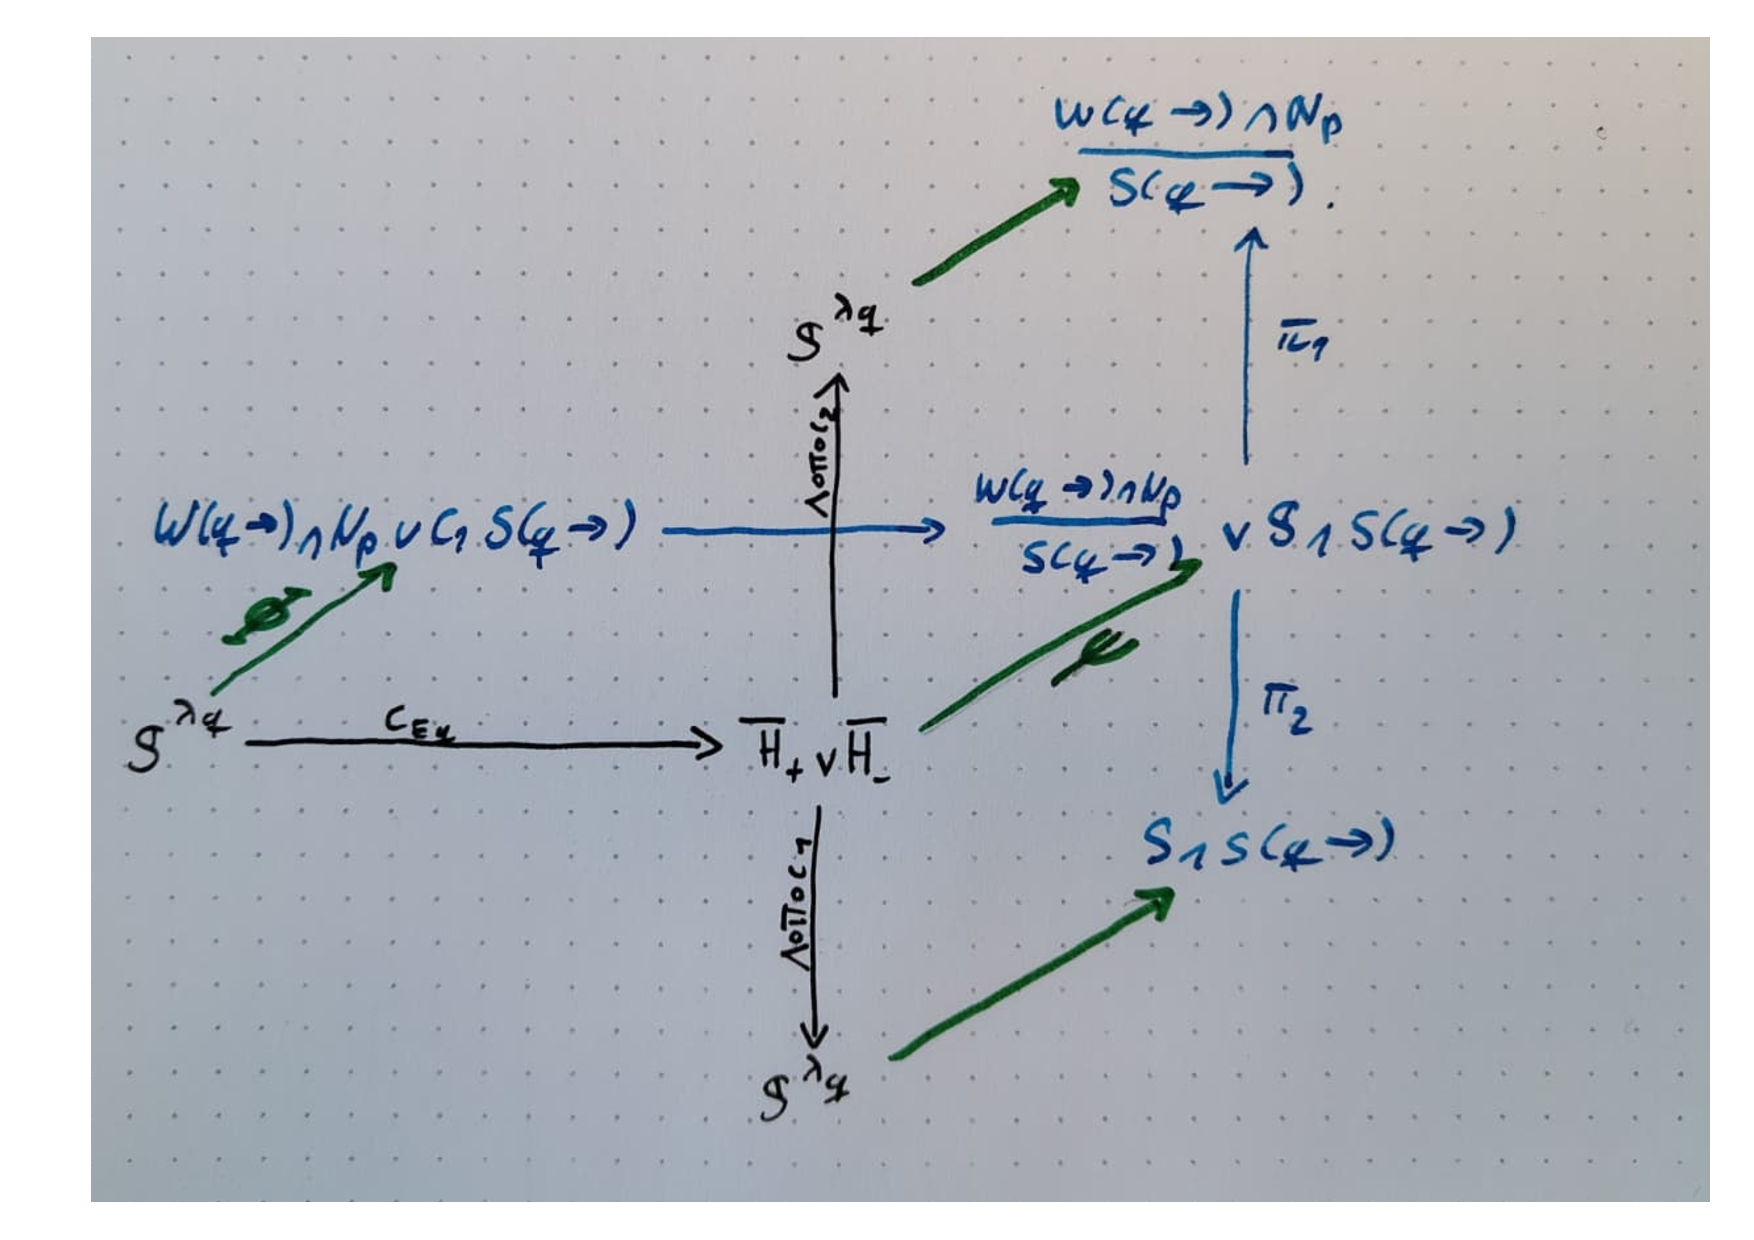
\includegraphics[width=\textwidth]{Text/Pictures/Kommutative Diagram Sphere equator collaps.jpeg.pdf}
			\end{fdiagram}
			Now define $r\coloneq -R$. For example apply $R$ after the reflection $(x_0,\dots x_{\lambda_q})\mapsto (-x_0,\dots,x_{\lambda_q})$. Then by the lemma above and commutativity we have up to homotopy:
			\begin{align*}
				r\circ f_q\circ k_1 
				&=  	-R\circ f_q\circ k_1 \circ \Phi \circ \Phi^{-1}\\
				&=  	-R\circ \Lambda \circ \pi\circ c_2\circ C_{Eq} \circ \Phi^{-1}\\
				&=  	R\circ \underbrace{\Lambda \circ \pi\circ c_1\circ C_{Eq} }_{\simeq \id}\circ\Phi^{-1}\\
				&=		col\, .
			\end{align*}
			
		\end{itemize}  
		With $r$ we finally have all the maps. Now we want to find out what degree the composition
		$s\circ r$ has. For this we calculate the local degree in some point by checking the sign of the determinant of the Jacobean. This strategy works out since we are in the situation of lemma \ref{lem: determined of javobean and collapsing map}.
		Bevor we start differentiating, we expand the map arround $x\in \R^{\lambda_q}$, such that $x'\coloneq E^u_q\circ B_{\mathfrak{b}^q}(x)\in \rho{-1}(x_j)$, meaning that $x'$ is on the flow line towards $x_j$ and assume that $\tau(x')=1$.
		\begin{align*}
			&   \phantom{=}	\pi_+\circ s\circ r\circ \pi_+^{-1}(x_1,\dots .,x_{\lambda_q})\\
			&=	\pi_+\circ s\circ R (- x_0,x_1,\dots .,x_{\lambda_q}) \quad x_0>0\\
			&=	\pi_+\circ s\circ col \circ \restr{\Phi}{H_-} (-x_0,x_1,\dots .,x_{\lambda_q}) \\
			&=	\pi_+\circ f_p\circ l_1 \circ col \left(e^{\tau(x')},\rho(x')\right) \quad \text{ $col$ and $l_q$ are the identity arround $\left(e^{\tau(x')},\rho(x')\right)$ } \\
			&=\pi_+\circ \Omega  \Big(e^{\tau(E^u_q\circ B_{\mathfrak{b}^q}(x))},\Gamma \circ \underbrace{B_{\mathfrak{b}^p}^{-1} \circ \nu_{x_j}\circ J^{-1}\circ \rho \circ E^u_q\circ B_{\mathfrak{b}^q}(x)}_{\coloneq Z(x)}\Big)\\
			&=\sin(\pi e^{\tau(E^u_q\circ B_{\mathfrak{b}^q}(x))}) \cdot
			\begin{pmatrix}
				-\cos\left(\pi \cdot \norm{Z(x)}\right)\\
				\sin\left(\pi \cdot \norm{Z(x)}\right) \cdot \frac{Z(x)}{\norm{Z(x)}})
			\end{pmatrix}
		\end{align*}
		Here $Z$ is a funktion $Z: \inti(I\times D^{\lambda_q})\to \R^{\lambda_q-1}$ and we can calculate its jacobean Notice how $Z(y)=0$ where $y$ is the same as above. We only care for the sign of its jacobean, so we will manipulate the funktion in a way that might change the function, but not the sign of ots Jacobean determinant. 
		Let $Q_y: V\to T_yV$ be the canonical map, that identifies a linear space with the tangendspace of a point from inside said space. Now we calculate:
		
		
		\begin{align*}
			&\phantom{=}Q_0^{-1}\circ \restr{\diff \left(B_{\mathfrak{b}^p}^{-1} \circ \nu_{x_j}\circ J^{-1}\circ \rho \circ E^u_q\circ B_{\mathfrak{b}^q}\right)}{y}\circ Q_y (e_i)\\
			&=Q_0^{-1}\circ  \restr{\diff \left(B_{\mathfrak{b}^p}^{-1} \circ \nu_{x_j}\circ J^{-1}\circ \rho \circ E^u_q\right)}{B_{\mathfrak{b}^q}(y)}\circ Q_{B_{\mathfrak{b}^q}(y)}\circ B_{\mathfrak{b}^q}(e_i) \\
			&= Q_0^{-1}\circ \restr{\diff \left(B_{\mathfrak{b}^p}^{-1} \circ \nu_{x_j}\circ J^{-1}\right)}{x_j}\circ \restr{\diff \left( \rho \circ E^u_q\right)}{B_{\mathfrak{b}^q}(y)}\circ Q_{B_{\mathfrak{b}^q}(y)}\circ B_{\mathfrak{b}^q}(e_i)		
		\end{align*}
		Now the term $\restr{\diff \left( \rho \circ E^u_q\right)}{B_{\mathfrak{b}^q}(y)}\circ Q_{B_{\mathfrak{b}^q}(y)}\circ B_{\mathfrak{b}^q}$ maps $e_1$ to zero. and $(e_2,\dots e_{\lambda_q})$
		induces a basis in $T_{x_j}V_j$ that is compatible with a basis $(\mathfrak{d}_i)_{i=2,\dots \lambda_q}$ that satisfies the following: Adding $-\grad_{x_j}(f)$ as the first basis vector to $(\mathfrak{d}_i)_{i=2,\dots \lambda_q}$ gives a basis of $T_{x_j}W(q\to)$ that is compatible with the basis induced from $\mathfrak{b}^q$ that appears in the counting of flow lines in the Morse boundary operator. This was proven earlyer in lemma \ref{lem: Rho and Tau induces a Morse boundary orientation}.
		Now we can look at the first part: 
		\begin{align*}
			Q_0^{-1}\circ \restr{\diff \left(B_{\mathfrak{b}^p}^{-1} \circ \nu_{x_j}\circ J^{-1}\right)}{x_j}
			&=\Big(\restr{\diff J}{x_j}\circ \restr{\diff \nu_{x_j}^{-1}}{0}\circ \restr{\diff B_{\mathfrak{b}^p}}{0} \circ Q_0 \Big)^{-1}\\
			&=\Big(\underbrace{\restr{\diff J}{x_j}\circ Q_{0}}_{=\id_{T_{x_j}V_j}} \circ \nu_{x_j}^{-1}  \circ B_{\mathfrak{b}^p} \Big)^{-1}\\	
			&=\Big( \nu_{x_j}^{-1}  \circ B_{\mathfrak{b}^p} \Big)^{-1}
		\end{align*}
		Notice how $\nu_{x_j}^{-1}  \circ B_{\mathfrak{b}^p}$ induces a basis on $T_{x_j}V_j$ from a basis in $T^u_pM$. Comparing this basis to the basis  $(\mathfrak{d}_i)_{i=2,\dots \lambda_q}$ is what assigned the sign to the flow line in the Morse boundary operator. By the calculations we know that the Jacobean of the funktion $Z$ 
		\begin{equation*}
			\diff Q_0^{-1}\circ \restr{\diff \left(B_{\mathfrak{b}^p}^{-1} \circ \nu_{x_j}\circ J^{-1}\circ \rho \circ E^u_q\circ B_{\mathfrak{b}^q}\right)}{y}\circ Q_y=
			\begin{pmatrix}
				0&\tilde{Z}
			\end{pmatrix}\,,
		\end{equation*}where $\tilde{Z}$ is a $\lambda_{q-1}$ matrix with the sign of its determinant being given by the sign in the Morse boundary operator $n_{\gamma}$. 
		
		Now we can calculate the differential 
		\begin{align*}
			&   \restr{\diff \Big( \pi_+\circ s\circ r\circ \pi_+^{-1}(x_1,\dots .,x_{\lambda_q})\Big)}{x}\\
			&=  \restr{\diff \left(\sin(\pi e^{\tau(E^u_q\circ B_{\mathfrak{b}^q}(x))}) \cdot
				\begin{pmatrix}
					-\cos\left(\pi \cdot \norm{Z(x)}\right)\\
					\sin\left(\pi \cdot \norm{Z(x)}\right) \cdot \frac{Z(x)}{\norm{Z(x)}})
				\end{pmatrix}\right)}{x}
		\end{align*} To keep it readable we will first calculate
		\begin{equation*} 
			\restr{	\diff \left(\sin(\pi e^{\tau(E^u_q\circ B_{\mathfrak{b}^q}(x))})\right)}{x}=\cos(\pi\cdot \euler )\cdot \pi \euler \cdot \restr{\diff \tau }{E^u_q\circ B_{\mathfrak{b}^q}(x)}=\Big(\underbrace{\cos(\pi\cdot \euler )\cdot \pi \euler}_{<0},0,\dots,0\Big) 
		\end{equation*} 
		In this calculation we used that $x$ was choosen such that $\tau\circ E^u_q \circ B_{\mathfrak{b}^q}=1$ and $\mathfrak{b}^q$ was such that $\restr{\diff E^u_q}{y}\circ Q_y(\mathfrak{b}^q_i)$ equals $-\grad_{y}(f)$ for $i=1$ and for $i>1$ it equals $\restr{\diff \phi_{\tau(y)}}{y}^{-1}({w_i})$ where $(w_i)$ denotes a basis of $T_{x_j}V_j$. Hence applying the product rule to the differential above yealds a sum with the first summond being
		\begin{equation*}
			\left(-1,0,\dots,0\right)\cdot 	\Big(\underbrace{\cos(\pi\cdot \euler )\cdot \pi \euler}_{<0},0,\dots,0\Big)^\top=
			\begin{pmatrix}
				a&0\\
				0&0
			\end{pmatrix} \, \quad \text{where  }a>0\,.
		\end{equation*} Here we just used, that $Z(x)=0$. The second summand is:
		\begin{equation*}
			\underbrace{\sin(\pi\cdot e)}_{>0}\begin{pmatrix}
				\sin(0)\cdot *=0\\
				\pi\cdot 1_{\lambda_q\times \lambda_q}\circ \restr{\diff Z}{x}
			\end{pmatrix}=\begin{pmatrix}
				0&0\\
				0&b\cdot Z
			\end{pmatrix}\quad \text{ where $b>0$)}\,.
		\end{equation*} Here we used that
		\begin{equation*}
			\restr{\diff \frac{\sin(\pi\norm{x})}{\norm{x}}\cdot x}{x\to 0}=\pi\cdot 1_{\lambda_q\times \lambda_q}
		\end{equation*} But with this we have the jacobean 
		\begin{equation*}
			\restr{\diff \Big( \pi_+\circ s\circ r\circ \pi_+^{-1}(x_1,\dots .,x_{\lambda_q})\Big)}{x}=\begin{pmatrix}
				a&0\\
				0&bZ
			\end{pmatrix}\,,
		\end{equation*} and know that its determinant has a positive that equals $n_{\gamma}$ which is the assigned sign to the flow line containing $x_j$ in the Morse Boundary operator. Or said differently: The local and hence global degree of the map $r^*\circ s^*$ equals $n_\gamma$. With this we can calculate 
		\begin{equation*}
			\delta^j_{triple}(\alpha_p)=\sum_{j}\delta^j_{triple}\circ f_p^*(\beta)=n_{\gamma}f^*_q(\beta)=n_\gamma(\alpha_q)
		\end{equation*}
		Furthermore: $\Delta(\alpha_p)=\delta^2_{triple}(\alpha_p)=\sum_{\gamma \in \mathcal{q,p}} n_\gamma(\alpha_q)$. This concludes the prove. 
	\end{proof}
	\begin{corollary} [Simplifying the Spectral Sequence]
		By the bott-periodicity we have natural isomorphisms between 
		\begin{equation*}
			\beta:	E^{p,q}_r\cong E^{p,p+2}_r\,,
		\end{equation*} and the commuting squares
		\begin{center}
			\begin{tikzcd}
				E^{p,q  }_q \arrow[r,"d_r^{p,q  }"] \arrow[d,"\beta"]&E^{p+r,q-r+1}_r \arrow[d,"\beta"]\\
				E^{p,q+2}_q \arrow[r,"d_r^{p,q+2}"]                &E^{p+r,q+2-r+1}_r
			\end{tikzcd}
		\end{center}
		By diagrramm \ref{diag: first page comparison} we know that $E_1^{*}$ is isomorphic to the following double graded group with a map: 
		\begin{center}
			\begin{framed}
				\begin{adjustbox}{width=\textwidth}
					% https://tikzcd.yichuanshen.de/#N4Igdg9gJgpgziAXAbVABwnAlgFyxMJZAZgBoBGAXVJADcBDAGwFcYkQBhAPWAAYBfABQBZUgB0xAW3o4AFgDMATvQDWwAIL9xYgFoBKEFvSZc+QigAsFanSat23YOSGiJ0uUtUatE-YdLG2HgERACs1jQMLGyInDwATC7a7grKaprafkYgGEFmRABsEbbR7BIAxlAQOAjZuaYhKGTxNlH2sbz+gQ3myFYtkXYxIJ11JsG94QMl7SNdOeP5KEXTbcMVVTXz9RNEZMStQw48AiLJMqleGb4GY3mNfaQHg6Wxjs5nbhee6T66twEFvdJk9Dq84sBEp8pN80t5MgDurtlqCXrMNtVaoCdksSKQLGDZqNsYsHlYCWjhsSkbjwhSZlTtqTekV6WsymJKpimcCiPFiuyOjyenzSKsjkK7iKUPzngz2NSgdLkPy2RK5lLkcheAL1cKtTrQoThvrceRdeCMVtNWaxcaOVzrSTeShzXLBSArViaQ9zWrLZzNt6lVrzbx7bFTQ8iuHKexDDYYFAAObwIigJQQSRIHUgHAQJDm+WxCRoeiKPBMLiKzPZxBF-NIfnFz1iMsVrBV8jzWtNmiNxBkFul8uVxhceI9xRZpAADn7BcQAE44yW26PO+Oa9O6yu84vyLmPSOO12pzP67mB+Qi8f16fx5Psr3EEV90gAOzPndIcLv1-fheVj-qEgF1uQzbXsQYGFkO14WDB9bAdeoGAi+5B7teiRoT+9bzv+s6IeQH4LkgCE4Re5BvgOAgUXW8RXou8S3uqACOIA0Iw9AAEYwIwAAKzLsIoWDJrIODnvRf7XkuiHxMhB6EXRTZwQeX7KYg8SQQeBRydRTEkS2aAJvwQA
					\begin{tikzcd}
						& {} \arrow[rrrrr, "p"] &             &                                                    &                                                    &                                                    & {}     \\
						{} \arrow[dddd, "q"'] & \cdots \arrow[r]      & 0 \arrow[r] & {C^{0}(M,\mathfrak{A},\Z)} \arrow[r, "\partial^0"] & {C^{1}(M,\mathfrak{A},\Z)} \arrow[r, "\partial^1"] & {C^{2}(M,\mathfrak{A},\Z)} \arrow[r, "\partial^2"] & \cdots \\
						& \cdots \arrow[r]      & 0 \arrow[r] & 0 \arrow[r]                                        & 0 \arrow[r]                                        & 0 \arrow[r]                                        & \cdots \\
						& \cdots \arrow[r]      & 0 \arrow[r] & {C^{0}(M,\mathfrak{A},\Z)} \arrow[r, "\partial^0"] & {C^{1}(M,\mathfrak{A},\Z)} \arrow[r, "\partial^1"] & {C^{2}(M,\mathfrak{A},\Z)} \arrow[r, "\partial^2"] & \cdots \\
						& \cdots \arrow[r]      & 0 \arrow[r] & 0 \arrow[r]                                        & 0 \arrow[r]                                        & 0 \arrow[r]                                        & \cdots \\
						{}                    &                       &             &                                                    &                                                    &                                                    &       
					\end{tikzcd}
				\end{adjustbox}
			\end{framed}
		\end{center}
		And hence, $E_2^{p,q}$ is isomorphic to the quotient 
		\begin{framed}
			\begin{center}
				\begin{adjustbox}{width=\textwidth}
					% https://tikzcd.yichuanshen.de/#N4Igdg9gJgpgziAXAbVABwnAlgFyxMJZAZgBoBGAXVJADcBDAGwFcYkQAJAPQAYAKALKkAOsIC29HAAsAZgCd6Aa2ABBAL4jhALQCUIDeky58hFABYK1Ok1btu5QZonT5S1RtG79pQ9jwEiAFZLGgYWNkROLgAmR1FnWQVldU0vAxAMPxMiADYQ63D2UQBjKAgcBHTM4wCUMmirMNtInm9fGtNkCwbQmwiQVqqjf07gnoLmgbaM4eyUPPGm-pKyiunqkaIyYka+u1448UlEtxTPPSGs2q7SHd7CyPtDhNdkj20Lnxmr0dvdh6isSE8WOr3cqU+7U28z+90mK3KlS+GzmJFIZn+k0GyNm1wsGLh-WxUNReQJE2WwlKiPWuM60XyS3YxO+HSIDMWexatJ+7NhFOZPLZKAZ5KZ3MuwuQPEZXJAQuh0tIgUx-QVqPIsoBCLWksVms52qpqyRJOumruAsiOtNrP16NVRWNNL1GtIPEdkXV1zyHsJ7G9vzFcsGVhgUAA5vAiKB5BAxEhyABOGg4CBIaIyq0gACOIBojHoACMYIwAAp09hyLARqQ4aZxhOIaLBEBpjN5bNoBtyeNICxt9PN9KNxOd9uIcgj3tN6IMwdIHjTvuIVsT4jL2dkBeIMybxMAdlTQ8C+8QAA5j0gcmeUzuD2fogOJ+ez+RLzuk2-5xPyEuvqOk7br+U6UGoQA
					\begin{tikzcd}
						& {} \arrow[rrrrr, "p"] &               &                                      &                                      &                          & {}     \\
						{} \arrow[dddd, "q"'] & \cdots                & 0             & {H^0(M,\mathfrak{A},\Z)}             & {H^1(M,\mathfrak{A},\Z)}             & {H^2(M,\mathfrak{A},\Z)} & \cdots \\
						& \cdots \arrow[rru]    & 0 \arrow[rru] & 0 \arrow[rru]                        & 0 \arrow[rru]                        & 0                        & \cdots \\
						& \cdots \arrow[rru]    & 0 \arrow[rru] & {H^0(M,\mathfrak{A},\Z)} \arrow[rru] & {H^1(M,\mathfrak{A},\Z)} \arrow[rru] & {H^2(M,\mathfrak{A},\Z)} & \cdots \\
						& \cdots \arrow[rru]    & 0 \arrow[rru] & 0 \arrow[rru]                        & 0 \arrow[rru]                        & 0                        & \cdots \\
						{}                    &                       &               &                                      &                                      &                          &       
					\end{tikzcd}
				\end{adjustbox}
			\end{center}
		\end{framed}
		Now since later pages are summand-wise quotients of earlyer pages we have that $E^{p,q}_r=0$ if $q$ is odd. This is also true for $E^{p,q}_{\infty}$, since the sequence stabilices, meaning that it becomes independent of $r$ for $r$ big enough. With this we do the following simplifications: 
		\begin{itemize}
			\item First we identify for all even $q$ $E^{p,q}_r$ with $E^{p,0}_r \equiv E^p_r$.
			\item If $r$ is even, then $d^{p,q}_r: E^{p,q}_r\to E^{p+r,q-r+1}_r$ is the trivial map, since the image is trivial. 
		\end{itemize} 
	\end{corollary}
	
	
	
	\begin{theorem}[The last page]
		The Last page $E^{pq}_{\infty}$ is in some sense associated top the K-groups
	\end{theorem}
	\begin{definition}[Filtration of the K-Groups]
		We define:
		\begin{equation*}
			\prescript{(r)}{}{K^p(M)}\coloneq \ker\left[i^*: K^p(M)\to K^p(N_r)\right]
		\end{equation*} With this we get the two filtrations:
		\begin{align*}
			&K^0(M)~=~	\prescript{(-1)}{}{K^0(M)} ~~\supseteq ~~\prescript{(0)}{}{K^0(M)}~~\supseteq~~ \prescript{(1)}{}{K^0(M)}~~\supseteq ~~\cdots~~ \supseteq ~~ \prescript{(m)}{}{K^0(M)}~=~0 \\
			&K^0(M)~=~	\prescript{(-1)}{}{K^1(M)} ~~\supseteq ~~\prescript{(0)}{}{K^1(M)}~~\supseteq~~ \prescript{(1)}{}{K^1(M)}~~\supseteq ~~\cdots~~ \supseteq ~~\prescript{(m)}{}{K^1(M)}~=~0
		\end{align*}
	\end{definition}
	\begin{lemma}
		Let $s\in 2\Z$ be even. Then:
		\begin{equation*}
			\prescript{(s)}{}{K^0(M)}=\prescript{(s+1)}{}{K^0(M)}\quad \text{and}\quad 	\prescript{(s-1)}{}{K^1(M)}=\prescript{(s)}{}{K^1(M)}
		\end{equation*}
	\end{lemma}
	\begin{proof}
		First we inspect the $K$ sequence of the triple $(M,N_{s+1},N_s)$:
		\begin{center}
			\begin{tikzcd}
				{	K^0(M,M_{s+1})} \arrow[r,"\epsilon \coloneq i^*"]&{K^0(M,M_{s})}  \arrow[r,"i^*"]& {\underbrace{K^0(M_{s+1},M_{s})}_{=0}}
			\end{tikzcd}
		\end{center}The last $0$ is a result of $(K^0(M_{s+1},M_{s})$ being an index pair of $\Crit_{s+1}$ and hence the quotient is homotopically equivalent to a bouquet of spheres of odd dimension. Hence taking the zeroth th K-group yealds the trivial group. But then $\epsilon$ is an epimorphism. Now since the square of inclusions is commutative:
		\begin{center}
			\begin{tikzcd}
				{(M,N_s)} \arrow[d]& \arrow[l] M \arrow[d]\\
				{(M,N_{s+1})}&\arrow[l] M
			\end{tikzcd}
		\end{center}
		We get the commutative ladder
		\begin{center}
			\begin{tikzcd}
				{K^0(M,N_s)} \arrow[r,"\alpha"]                        & K^0(M)\arrow[r,"\beta"] \arrow[d, equal ] &K^0(N_{s+1})&\quad \text{long exact sequence of }(M,N_s)\\
				{K^0(M,N_{s+1})} \arrow[u,"\epsilon"]\arrow[r,"\gamma"]& K^0(M)\arrow[r,"\delta"]& K^0(N_{s+1})&\quad \text{long exact sequence of }(M,N_{s+1})
			\end{tikzcd}
		\end{center} Now from $\epsilon$ being an epimorphism we can conclude that the image of $\alpha$ equals the image of $\gamma$ and hence the kernel of $\beta$ agrees with the kernel of $\delta$. This concludes the first part of the lemma. The second part is proven by the same argument. 
	\end{proof}
	With this we can simplyfy the gradings:
	\begin{align*}
		I: 	K^0(M)~=~\prescript{(0)}{}{K^0(M)}~\supseteq~\prescript{(2)}{}{K^0(M)}~\supseteq~\prescript{(4)}{}{K^0(M)}~\supseteq ~\cdots~\supseteq 0\\ 
		J: K^1(M)~=~\prescript{(-1)}{}{K^1(M)}~\supseteq~\prescript{(1)}{}{K^1(M)}~\supseteq~\prescript{(3)}{}{K^0(M)}~\supseteq ~\cdots~\supseteq 0
	\end{align*}
	To find the last page $E^{p,q}_{\infty}$ we notice that for $r$ big enough, $N_{p+r-1}=M$ and $N_{p-r}=0$. Hence the spectral sequence becomes stationary with 
	\begin{equation*}
		E^{p,q}_{\infty}=\frac{\ker[K^{p+q}(M)\to K^{p+q}(N_{p-1})]}{\ker[K^{p+q}(M)\to K^{p+q}(N_{p})]}\,.
	\end{equation*}
	
	
	
